\documentclass[10pt,letterpaper,titlepage]{article}
\usepackage[latin1]{inputenc}
\usepackage{amsmath}
\usepackage{amsfonts}
\usepackage{amssymb}
\usepackage{gensymb}
\usepackage{geometry}
\usepackage{graphicx}
\usepackage{hyperref}
\usepackage{placeins}
\geometry{letterpaper, portrait, margin=1.25in}
\hypersetup{colorlinks=true,linkcolor=blue,urlcolor=blue}
\graphicspath{{images/}}
\author{Matt Gill}
\begin{document}
	\begin{titlepage}
		\begin{center}
			\vspace*{1cm}
            
\includegraphics[width=0.8\textwidth]{accupatt_logo.png}\\
			\vspace{0.5cm}
			\textbf{Aircraft Spray Pattern Testing Software}\\
			User Manual - Version 2.0.x
			\vfill
			\textbf{Developed By:}\\
			Matt Gill - University of Illinois\\
            \vspace{0.5cm}
			\textbf{Based on Previous Work By:}\\
			Dr. Richard Whitney - WRK of Oklahoma\\
			Phil Jank - USDA Aerial Application Technology Research Unit\\
            \vspace{0.5cm}
			\textbf{Aided Significantly by the Technical Expertise Of:}\\
			Dr. Scott Bretthauer - National Agricultural Avaition Association\\
            Dr. Brad Fritz - USDA Aerial Application Technology Research Unit\\
            Dr. Dennis Gardisser - WRK of Arkansas\\
		\end{center}
	\end{titlepage}
	\tableofcontents
	\newpage
	
    \section{Introduction}
	\textit{AccuPatt} is a desktop application created to process spray pattern data for agricultural aircraft. This includes measuring tracer dye deposition on string collectors and measuring droplet deposition from spray cards. The goals of this application are twofold:
    \begin{itemize}
        \item Maximize flexibility through parameterization to provide broad utility
        \item Wherever possible, simplify; The best tools don't need user manuals (And yet here we are)
    \end{itemize}

    \newpage

    \section{Compaitble Hardware}

    \subsection{String Hardware}
    To collect relative fluorescence deposition data from a linear (string) collector, special hardware is required. Specifically: 
    \begin{itemize}
        \item A light source of the excitation wavelength for the intended tracer dye
        \item A means to measure intensity of the emitted wavelength for the intended tracer dye
        \item A controlled means of moving the string through the excitation/emission point
    \end{itemize}
    Currently there are two systems available to accomplish this:
    \begin{itemize}
        \item{\textit{WRK System:}} The \textit{WRK of Oklahoma} String Spectrometer System is commercially available for purchase, and is the system that this software was originally built for. It uses a combination wavelength-specific LED and Band-Pass filter as the excitation source and a commercial USB Spectrometer (Ocean Optics, USB2000+ or Flame) as the emission wavelength measurement device. It utilizes a set of serially controlled stepper motors in conjunction with various clutches and pulleys to move the string at a constant speed. Any questions on the \textit{WRK of Oklahoma} system should be directed to its creator, Dr. Richard Whitney (\href{mailto:whitney3451@att.net}{whitney3451@att.net})
        \item{\textit{USDA-ARS AATRU System:}} The \textit{USDA} String Spectrometer System is not commercially avaialable, however, build specifications, a parts list and build instructions are freely available. It uses a combination wavelength-specific LED and Band-Pass filter as the excitation source and a commercial USB Spectrometer (Ocean Optics, USB2000+ or Flame) as the emission wavelength measurement device. It utilizes a variable-speed controller to drive a lightly-modified portable drill, with a rotary encoder providing feedback for PID control. Any questions on the \textit{USDA} system should be directed to its creator, Phil Jank (\href{mailto:phil.jank@usda.gov}{phil.jank@usda.gov}).
    \end{itemize}
    \textbf{\color{red}Note: Currently, only the WRK System is supported within AccuPatt. Compatibility with the USDA system is planned, but the timeline is uncertain.\color{black}}

    \subsection{Spray-Card Hardware}
    To process spray-cards, they must first be scanned with a flatbed scanner. It is recommended to use a dedicated scanner (not a combination printer/scanner) for the highest quality. A supported resolution of at least 1200 dpi is recommended for most applications. \textit{AccuPatt} does not communicate with the scanner. Instead, images are scanned using the software of your choice (typically that which comes with the scanner itself) and those images can be uploaded to \textit{AccuPatt} for processing.
    
    \newpage

    \section{Installation}

    \subsection{Windows}
    After downloading the installer, double click it to launch the install wizard. You will have the option to create a desktop shortcut if desired. 

    \subsection{MacOS}
    After downloading the .dmg file, double click it to open it as a volume. Drag the \textit{AccuPatt} icon to the \textbf{Applications} shortcut icon. 

    \newpage

    \section{Operational Overview}
    
    \subsection{New Series}
    All data and operations in \textit{AccuPatt} require a series. To acquire new data, a new series must be created. From the menubar, use \textbf{File $\rightarrow$ New Series} to view options available (Figure~\ref{fig:new_series}). A series is created with the user-defined default number of passes.
    \begin{itemize}
        \item \textbf{New Series $\rightarrow$ New Aircraft:} Create an empty series with required parameters set to default values.
        \item \textbf{New Series $\rightarrow$ File Aircraft:} Create a series, copying all application info from a previous data file. Increments the series number by 1. A list of previous data files in your current working directory will appear in the menu for you to select from. Alternatively, choosing \textbf{Select File Aircraft} will open a File Chooser allowing you to select a datafile from anywhere.
    \end{itemize}
    \begin{figure}[hb]
        \centering
        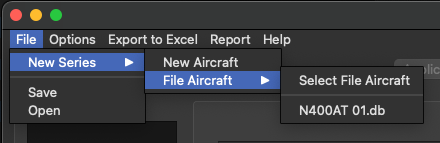
\includegraphics[width=0.6\textwidth]{new_series}
        \caption{New Series}
        \label{fig:new_series}
    \end{figure}
    
    \subsection{Application Info}
    It is generally desirable, but not required, to enter in some amount of information about the aircraft, spray system configuration, and/or applicator information to accompany pattern testing data. The \textbf{Application Info} tab provides fields to facilitate this (Figure~\ref{fig:application_info}). See the \hyperref[sec:data]{Data Structure} section for more details on specific fields.
    \begin{figure}[hb]
        \centering
        \makebox[\textwidth]{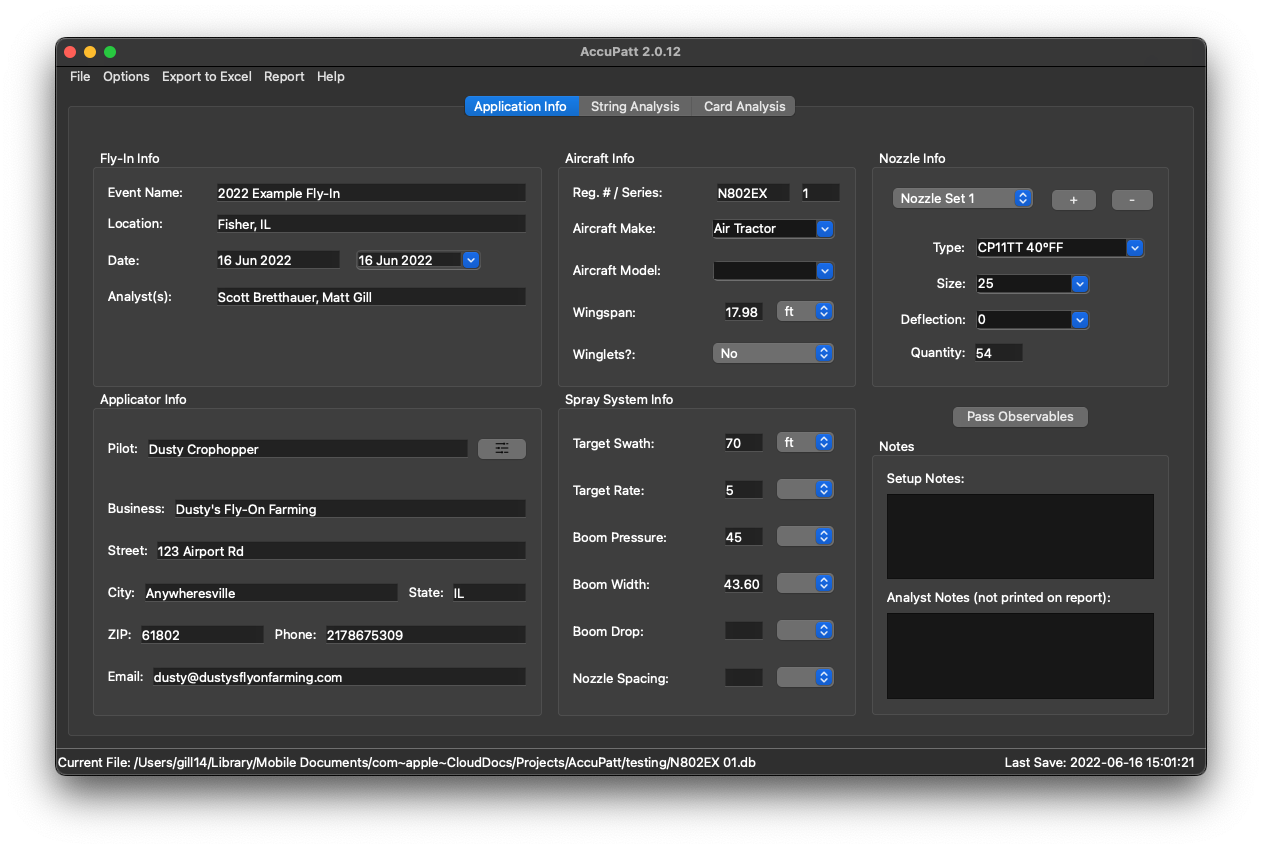
\includegraphics[width=\textwidth]{application_info.png}}
        \caption{Application Info Tab}
        \label{fig:application_info}
    \end{figure}
    \FloatBarrier

    \subsubsection{Pass Observables}
    In addition to \textbf{Application Info}, which is collected on a per-series basis, there is some observable data which is typically collected on a per-pass basis. These are frequently referred to here and in the program as \textbf{Pass Observables} since they consist solely of measured values obtained at the time of the application.\par
    These values can be entered in several locations for the convenience of the analyst. Typically, they are entered from either the \textbf{Capture/Edit String} winodw or the \textbf{Card Manager} window for any individual pass. Alternatively, choosing \textbf{Options $\rightarrow$ Pass Manager} from the menu will open the \textbf{Pass Manager} window (Figure~\ref{fig:pass_manager}) which contains a table with rows for each pass and columns for each pass observable parameter. In addition to the editable fields for pass observables, the pass name itself may be changed here. There are also checkboxes to facilitate the inclusion/exclusion of string and/or card data from series-wise calculations and plots.\par
    The \textbf{Pass Manager} window also provides buttons to add or remove passes from the series. There is no functional limit to the number of passes per series. A checkbox is provided which, if checked, will update the default number of passes to add to all future series.
    \begin{figure}[hb]
        \centering
        \makebox[\textwidth]{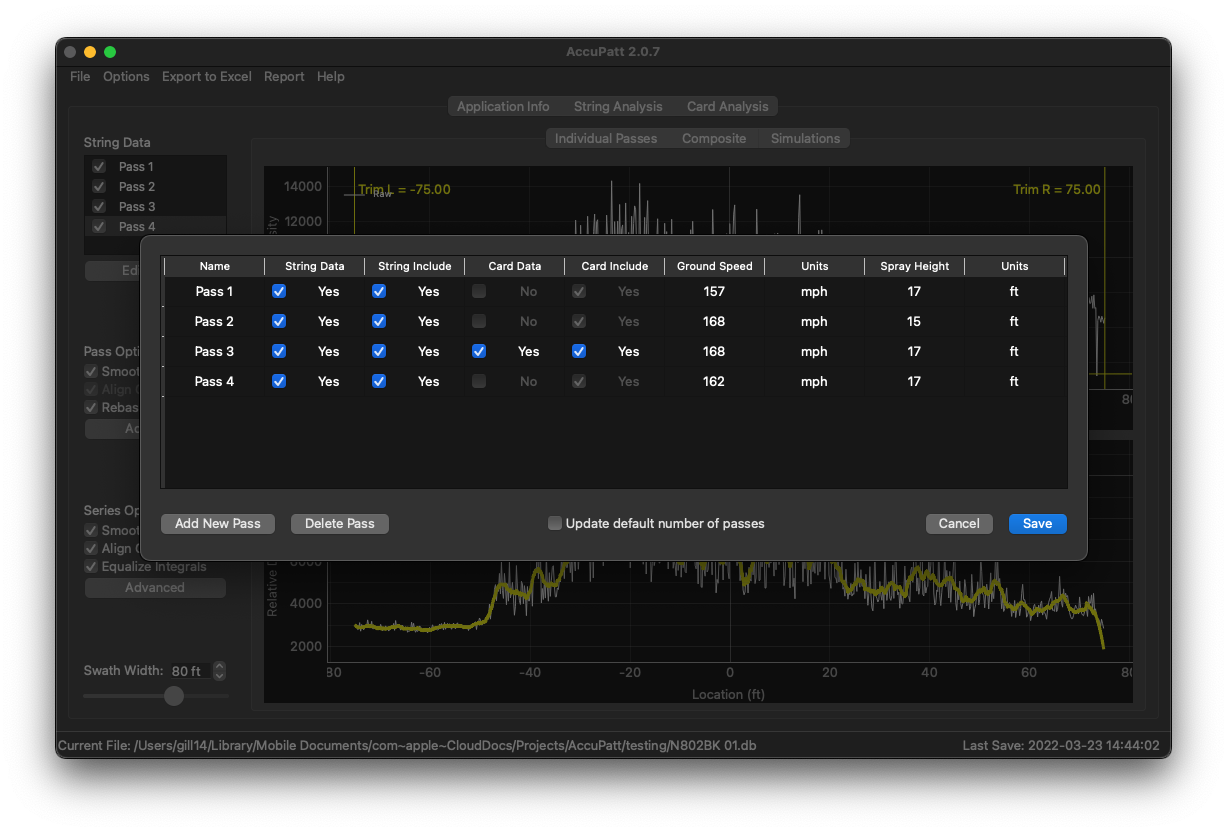
\includegraphics[width=\textwidth]{pass_manager.png}}
        \caption{Pass Manager}
        \label{fig:pass_manager}
    \end{figure}
    \newpage

    \subsection{String Analysis}
    String data is collected on a per-pass basis, but may be analyzed on a per-series basis. The \textbf{String Analysis} tab provides a list of passes in the series and pass/series processing options. This tab also contains sub-tabs for viewing/modifying data as discussed below.
    
    \subsubsection{Capture Pass}
    Choose the pass to be collected from the list of passes, then click the \textbf{Capture Pass} button. This will open the \textbf{Capture/Edit Pass} window (Figure~\ref{fig:capture_edit_pass}).\par
    This window provides indicators for the connection status of the string drive and spectrometer, with access to modify their settings (see the \hyperref[sec:string_hardware_settings]{String Hardware System Settings} section for more details).\par
    This window also provides optional data entry fields for observables specific to the applicable pass.\par
    If both the string drive and spectrometer are connected, clicking the \textbf{Start} button will engage the string drive, advancing the string, and simultaneously will change its text to \textbf{Mark}. Clicking the \textbf{Mark} button will begin the collection of spectrometer data at intervals specified by the set \textbf{integration time}. Data will continue to be collected until the set \textbf{string length} is reached. At any time after data collection is begun, clicking the \textbf{Abort} button will stop the string drive and clear all data collected up to that point.\par
    The \textbf{Clear} button may be used to clear the pass collected string data whenever data collecation is not in progress. If string data exists for the current pass, it will ask for confirmation first.
    \begin{figure}[h]
        \centering
        \makebox[\textwidth]{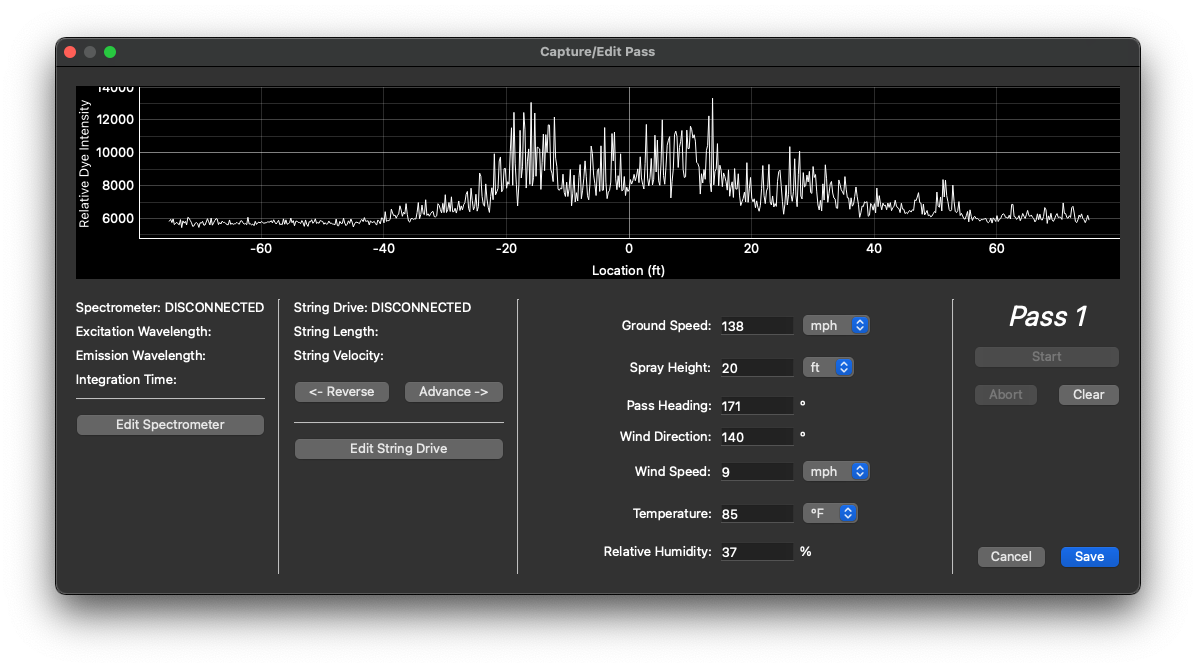
\includegraphics[width=\textwidth]{capture_edit_pass.png}}
        \caption{Capture/Edit Pass Window}
        \label{fig:capture_edit_pass}
    \end{figure}
    \newpage

    \subsubsection{View \& Trim Pass}
    Once string data for a pass is collected, the pass will have a check next to it in the pass list on the \textbf{String Analysis} tab. When a pass with string data is selected from the pass list, the \textbf{Individual Passes} sub-tab will show two plots (Figure~\ref{fig:string_individual}): 
    \begin{itemize}
        \item \textbf{Raw Data:} [Upper Plot] Plots data exactly as acquired. \textbf{Trim L} and \textbf{Trim R} (yellow) handles can be moved to exclude data outside their limits. The \textbf{Floor} handle will automatically be set to the lowest non-excluded data point, however, it may be further raised to pull up lower data points to a new level. This is typically done for subjectively removing background noise.
        \item \textbf{Modified Data:} [Lower Plot] Plots trimmed and rebased data (white) and overlays that with a copy which has had a smoothing filter applied (yellow). Rebasing and smoothing are only shown when applicable (see \hyperref[sec:string_options]{String Options})
    \end{itemize}
    \begin{figure}[h]
        \centering
        \makebox[\textwidth]{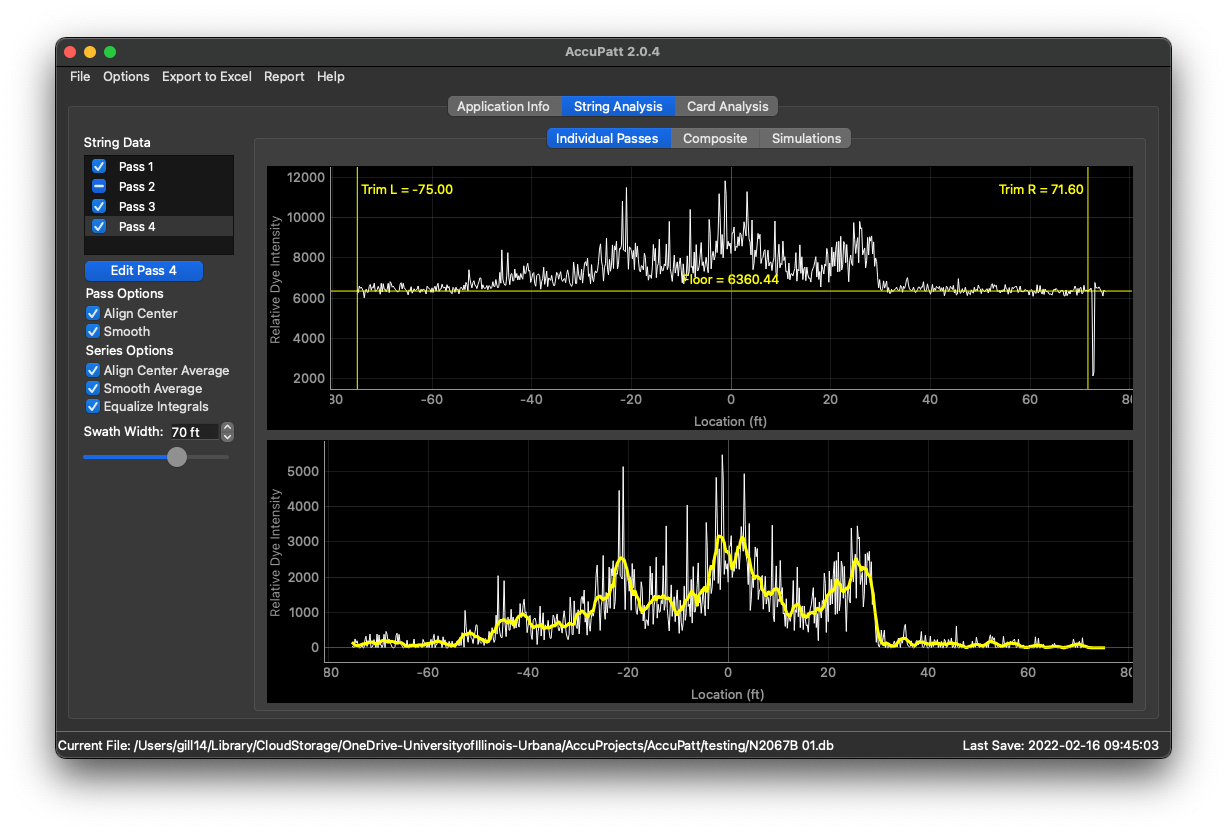
\includegraphics[width=\textwidth]{string_individual.png}}
        \caption{String Analysis - Individual Passes}
        \label{fig:string_individual}
    \end{figure}
    \newpage

    \subsubsection{Composite}
    The \textbf{Composite} sub-tab contains two plots (Figure~\ref{fig:string_composite}):
    \begin{itemize}
        \item \textbf{Overlay:} [Upper Plot] Each individual (non-excluded) pass is plotted together. 
        \item \textbf{Average:} [Lower Plot] Each individual (non-excluded) psss is used to generate an average pattern. A gray swath-box is plotted with x-bounds on the adjusted swath width. The height of the swath-box is equal to half the average integrated area under the bounded section of the average pattern.
    \end{itemize}
    \begin{figure}[hb]
        \centering
        \makebox[\textwidth]{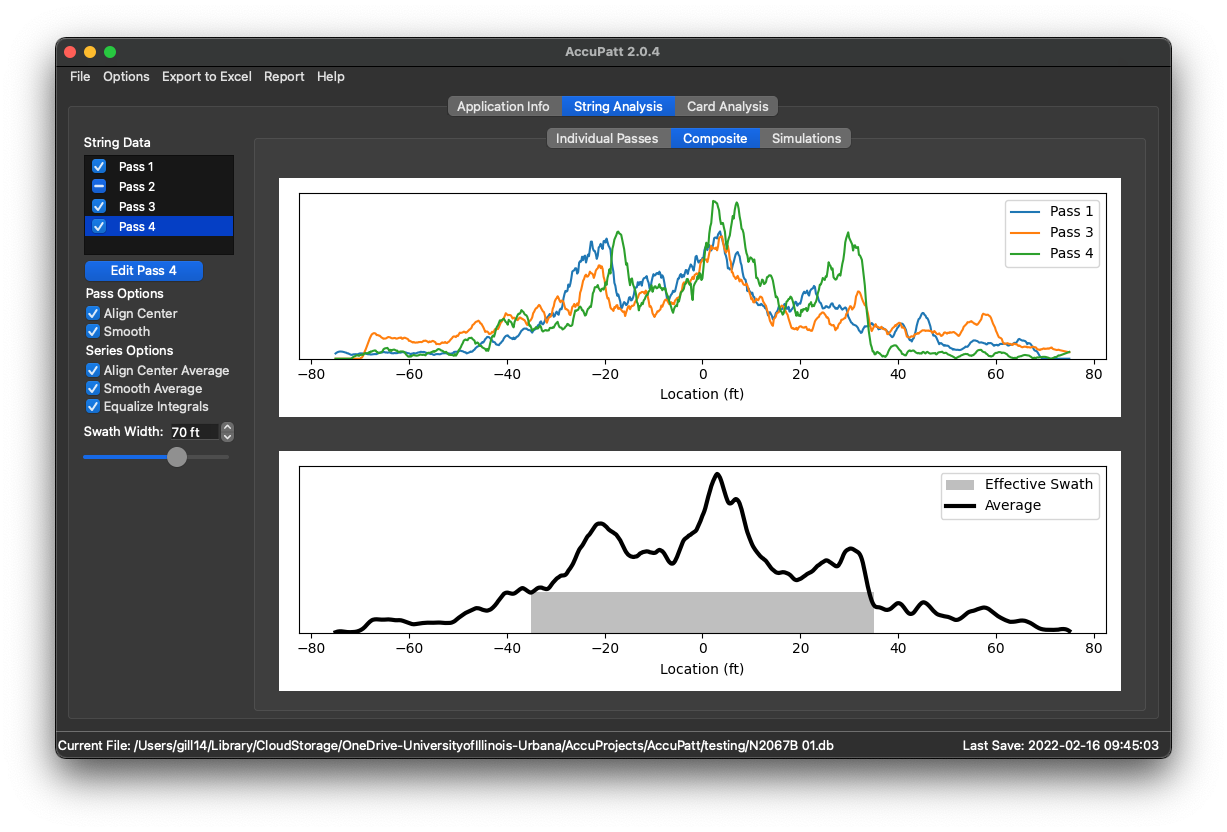
\includegraphics[width=\textwidth]{string_composite.png}}
        \caption{String Analysis - Composite}
        \label{fig:string_composite}
    \end{figure}
    \newpage

    \subsubsection{Options}
    \label{sec:string_options}
    The \textbf{String Analysis} tab contains \textbf{Pass Options} which affect only the selected pass:
    \begin{itemize}
        \item \textbf{Include In Composite:} Once a pass is recorded, a checkmark will appear adjascent to it in the pass list. This indicates that it is recorded and included in composite (series-wise) calculations and plots. Clicking the checkmark will turn it into a dash, indicating that it is recorded, but excluded ffom composite calculations and plots.
        \item \textbf{Smooth:} Apply smoothing filter to pass
        \item \textbf{Align Center:} Shift pattern left/right using chosen center method.
        \item \textbf{Rebase to X-Trim:} Recalculate each data point location such that the trimmed length is equal to the captured string length. If string speed is slightly faster than originally calibrated, this facilitates post-process correction to ensure accurate swath measurement.
        \item \textbf{Advanced Options:} Opens a popup with the following options:
        \begin{itemize}
            \item \textbf{Smoothing Window:} X-domain based distance over which the sliding smoothing filter is fit and applied
            \item \textbf{Smoothing Order:} Polynomial order for smoothing filter
            \item \textbf{Center Method:} Choose whether to center the pattern with the centroid or Center of Distribution.
        \end{itemize}
    \end{itemize}
    The \textbf{String Analysis} tab also contains \textbf{Series Options} which can apply to all passes and/or the average pattern:
    \begin{itemize}
        \item \textbf{Smooth Average:} Apply smoothing filter to average pattern
        \item \textbf{Align Center Average:} Shift average pattern left/right using chosen center method.
        \item \textbf{Equalize Integrals:} Scale each pass to the same integrated area
        \item \textbf{Advanced Options:} Opens a popup with the following options:
        \begin{itemize}
            \item \textbf{Smoothing Window:} X-domain based distance over which the sliding smoothing filter is fit and applied
            \item \textbf{Smoothing Order:} Polynomial order for smoothing filter
            \item \textbf{Center Method:} Choose whether to center the pattern with the centroid or Center of Distribution.
        \end{itemize}
    \end{itemize}
    The \textbf{String Analysis} tab also contains controls for setting the \textbf{Adjusted Swath Width} which defaults to the target swath width, but is saved independently.
    \newpage

    \subsubsection{Simulations}
    The \textbf{Simulations} sub-tab contains two plots (Figure~\ref{fig:string_simulations}). Both plots simulate overlapping the measured pattern at intervals of the desired swath width. The upper plot simulates use of a racetrack pattern and the lower plot simulations use of a back \& forth pattern. To simulate the back \& forth pattern, adjascent passes are mirrored about the center for odd passes. \color{red} The back \& forth simulation will not accurately represent in-field uniformity if the base pattern is obtained in a crosswind. \color{black}\par
    The number of \textbf{simulated adjascent passes} (each side) can be set to any non-negative integer.\par
    The plots can be drawn in \textbf{One Pass} mode, which will show only the mathematically relevant portion of the simulated overlap, specifically datapoints between -swathwidth/2 and swathwidth/2. Alternatively, the plots can be drawn in \textbf{All Passes} mode, which can be useful for illustrating the big picture of in-field overlap.\par
    The plotted area shows the additive contribution of all selected overlapping passes to the central swath width of the central pattern. The summation of all overlapped passes represents theoretical uniformity in the field and is used to compute the Coefficient of Variation (CV).\par
    The dashed horizontal line represents the average relative deposition about which standard deviations are computed for the CV calculations. In other words, the further each additive overlap point is from the average, the more it contributes to the overall CV.
    \begin{figure}[hb]
        \centering
        \makebox[\textwidth]{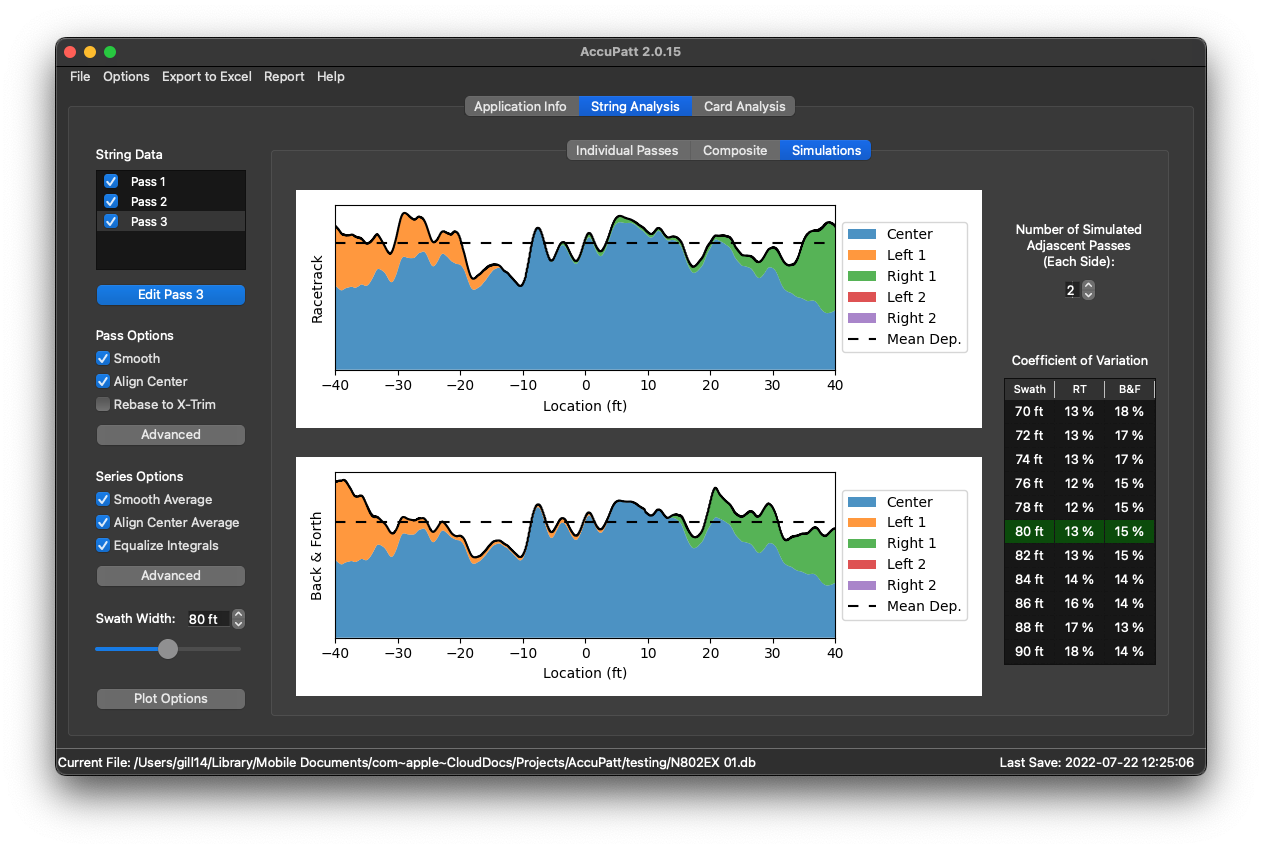
\includegraphics[width=\textwidth]{string_simulations.png}}
        \caption{String Analysis - Simulations}
        \label{fig:string_simulations}
    \end{figure}
    \newpage

    \subsection{Spray-Card Analysis}
    Card data is collected on a per-pass basis, but may be analyzed on a per-card or per-series basis as well. The \textbf{Card Analysis} tab provides a list of passes in the series and a list of cards declared in the selected pass. This tab also contains sub-tabs for viewing/modifying data as discussed below.

    \subsubsection{Capture Cards}
    \textit{AccuPatt} does not provide any functionality for digitizing spray-cards; instead, images acquired by the scanning software of your choice can be uploaded, saved to the datafile and used for further processing.\par
    In the \textbf{Card Analysis} tab, click the \textbf{Add/Edit Cards} button to open the \textbf{Card Manager} window (Figure~\ref{fig:card_manager}).\par 
    \begin{figure}[h]
        \centering
        \makebox[\textwidth]{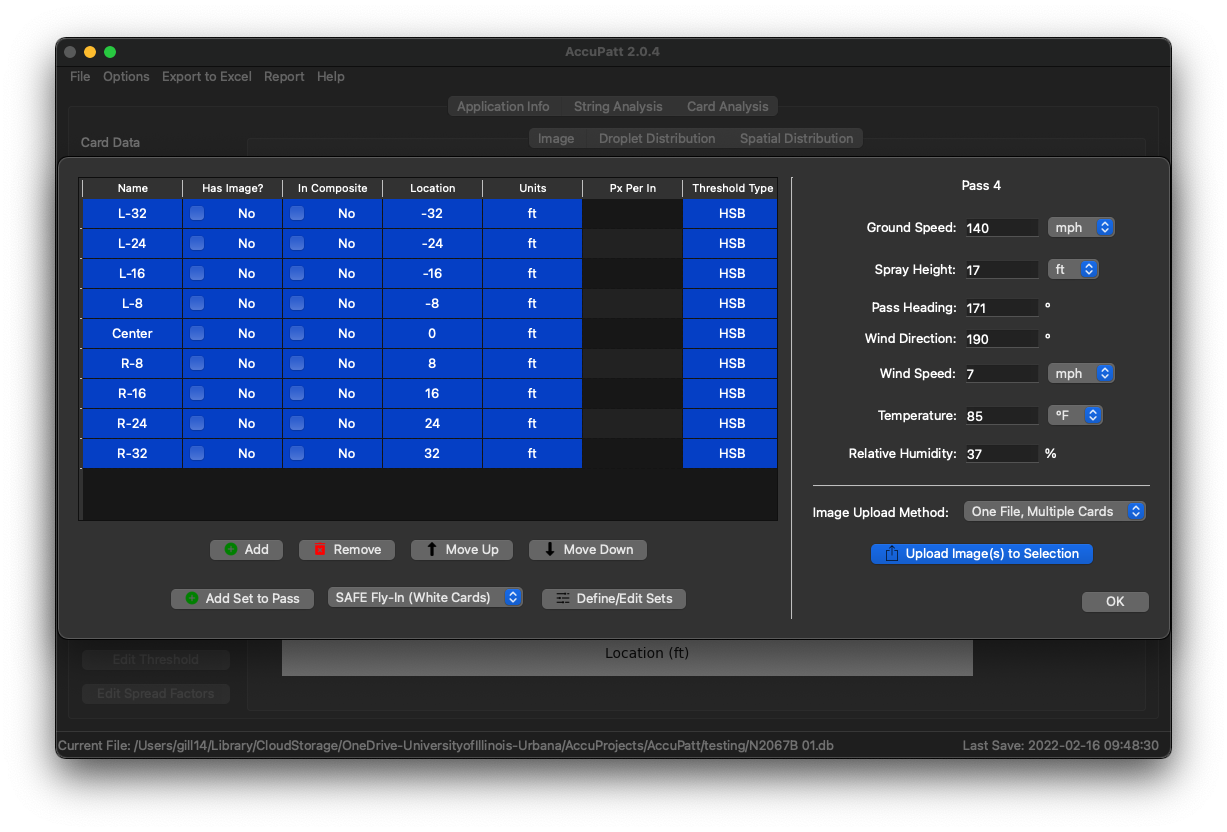
\includegraphics[width=\textwidth]{card_manager.png}}
        \caption{Spray-Card Analysis - Add/Edit Cards}
        \label{fig:card_manager}
    \end{figure}
    The \textbf{Card Manager} window provides a table of card data, with each row representing a card and each column a property of that card. properties may be edited by either double-clicking on them or utilizing provided checkboxes as applicable.\par
    Rows may be selected individually or by click-dragging over multiple rows. There are 4 buttons below this table:
    \begin{itemize}
        \item \textbf{Add:} Adds a new card in the last row, with default settings.
        \item \textbf{Remove:} Removes all selected cards. If any selected cards have image data in the datafile, a confirmation will appear prior to removal.
        \item \textbf{Shift Up:} Shift selected cards up by one row, if possible
        \item \textbf{Shift Down:} Shift selected cards down by one row, if possible.
    \end{itemize}
    Below these buttons are controls for utilizing \textbf{Defined Sets} which facilitate adding a pre-configured list of spray-cards to the list. Use the dropdown to select a set and click \textbf{Add Set To Pass} to append the cards to the table. More details can be found in the \hyperref[sec:defined_sets]{Defined Sets} section.\par
    To the right of the card table is a set of text fields for entering in observables for the current pass. These observables are shared between string and card data on the same pass. See the \hyperref[sec:data]{Data Structure} settings for more details.\par
    Below the pass observable entry fields are controls to \textbf{Upload Images} to the selected cards in the table. A dropdown facilitates choice of the upload method and and clicking the \textbf{Upload Image(s) to Selection} button will open a file chooser window to select all applicable files. A more detailed description of image upload methods and their processes can be found in the \hyperref[sec:image_upload]{Spray-Card - Image Upload} section.\par
    Once satisfied with the properties in the card table and with images uploaded, click \textbf{Ok} to return to the main window.
    \FloatBarrier

    \subsubsection{Check Image Processing}
    The \textbf{Image} sub-tab contains two image-views for the selected spray-card (Figure~\ref{fig:card_image}):
    \begin{itemize}
        \item \textbf{Stain Mask:} [Left Image] The original image forms the base layer. All stains have their perimeter outlined.
        \item \textbf{Stain Categorized:} [Right Image] A blank image with stains drawn (filled) and colored according to the following:
        \begin{itemize}
            \item \textbf{Undersize:} Not counted toward coverage or droplet spectrum analysis.
            \item \textbf{Edge:} Counted toward coverage, but not droplet spectrum analysis.
            \item \textbf{Valid:} Counted toward coverage and droplet spectrum analysis.
        \end{itemize}
    \end{itemize}
    The purpose of these views is to subjectively verify the image processing efficacy. To adjust image processing options click the \textbf{Edit Threshod} button. For more details, see the \hyperref[sec:image_process]{Image Process Options} section.\par
    By default, the image is scaled to fit the view horizontally; scrolling either image view will have the other follow in sync. Alternatively, the image-views can be set to scale the image to fit the vertical space using the control below the image-views.
    \begin{figure}[hb]
        \centering
        \makebox[\textwidth]{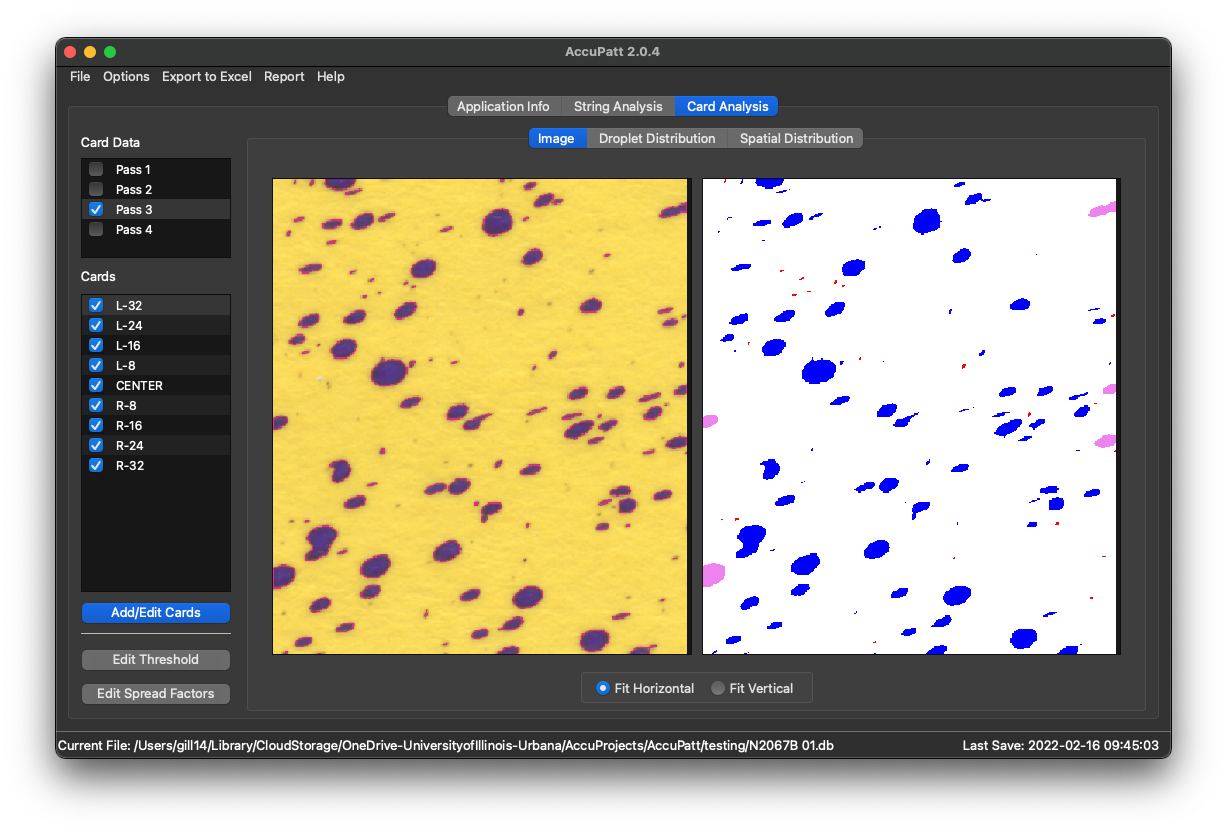
\includegraphics[width=\textwidth]{card_image.png}}
        \caption{Spray-Card Analysis - Image}
        \label{fig:card_image}
    \end{figure}
    \FloatBarrier

    \subsubsection{Droplet Distribution}
    The \textbf{Droplet Distribution} sub-tab contains two histogram plots (Figure~\ref{fig:card_droplet_dist}):
    \begin{itemize}
        \item \textbf{Spray Volume Contribution:} [Upper Plot] After discretizing the droplet spectrum, shows how much relative spray volume is contained in droplets of each discrete bin.
        \item \textbf{Quantity:} [Lower Plot] After discretizing the droplet spectrum, shows how many droplets of each discrete bin are found.
    \end{itemize}
    A table to the right of the histogram plots contains some select labeled droplet spectrum statistics.\par
    \color{red} The droplet spectrum category provided by \textit{AccuPatt} is based on reference nozzle laser diffraction measurements by USDA ARS. Because the measurement method is different the provided droplet spectrum category should not be considered absolute.\color{black}\par
    A dropdown menu at the upper-right facilitates selection of the scope of calculation. Depending on what pass and card is selected, you will see the following options if available:
    \begin{itemize}
        \item \textbf{Card:} Performs droplet analysis for the selected card only.
        \item \textbf{Pass:} Computes a representative composite card from all cards in the pass which have images and are not actively excluded, then performs a droplet analysis on that composite card. This is NOT simply a pass-wise average of single card statistics.
        \item \textbf{Series:} Same as \textbf{Pass}, except including cards from all (non-excluded) passes.
    \end{itemize}
    \begin{figure}[hb]
        \centering
        \makebox[\textwidth]{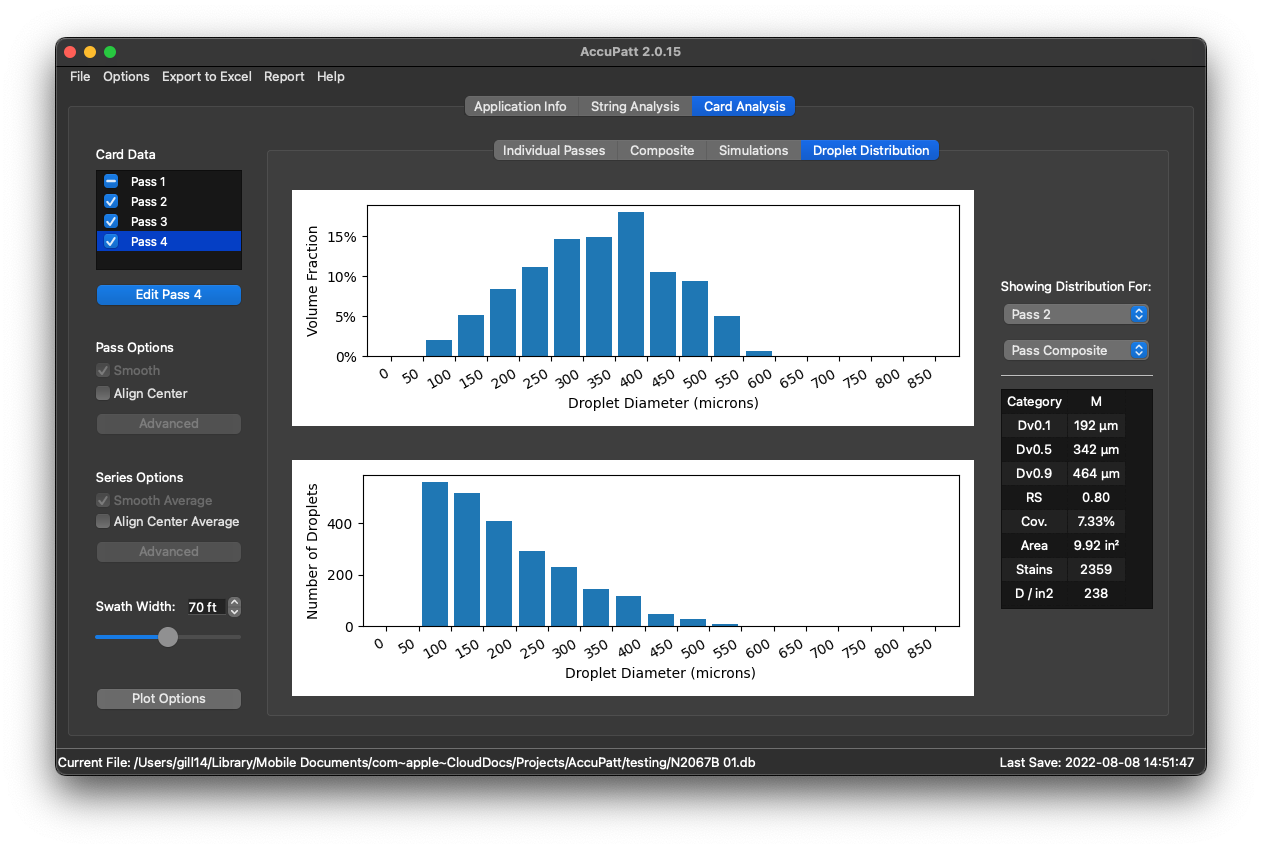
\includegraphics[width=\textwidth]{card_droplet_dist.png}}
        \caption{Spray-Card Analysis - Droplet Distribution}
        \label{fig:card_droplet_dist}
    \end{figure}
    \FloatBarrier

    \subsubsection{Spatial Distribution}
    The \textbf{Spatial Distribution} sub-tab contains two plots (Figure~\ref{fig:card_spatial_dist}):
    \begin{itemize}
        \item \textbf{Volume Fraction by Location:} For each card location, plots Dv0.1, Dv0.5 (VMD) and Dv0.9
        \item \textbf{Coverage by Location} For each card location, plots the percent coverage.
    \end{itemize}
    The \textbf{Plot X-Units} selection is available to rescale the plot axes to a unit other than what is declared with the card.\par
    The \textbf{Colorize by DSC} checkbox enables shading of the coverage plot with semi-standard droplet spectrum category colors. \color{red}This DSC shading utilizes linear interpolation of $D_{V0.1}$ and $D_{V0.5}$ between measured data points and recalculates the DSC for each interpolated location. This may result in DSC's shown between measured datapoints which do not actually exist in the measured data.\color{black}
    \begin{figure}[hb]
        \centering
        \makebox[\textwidth]{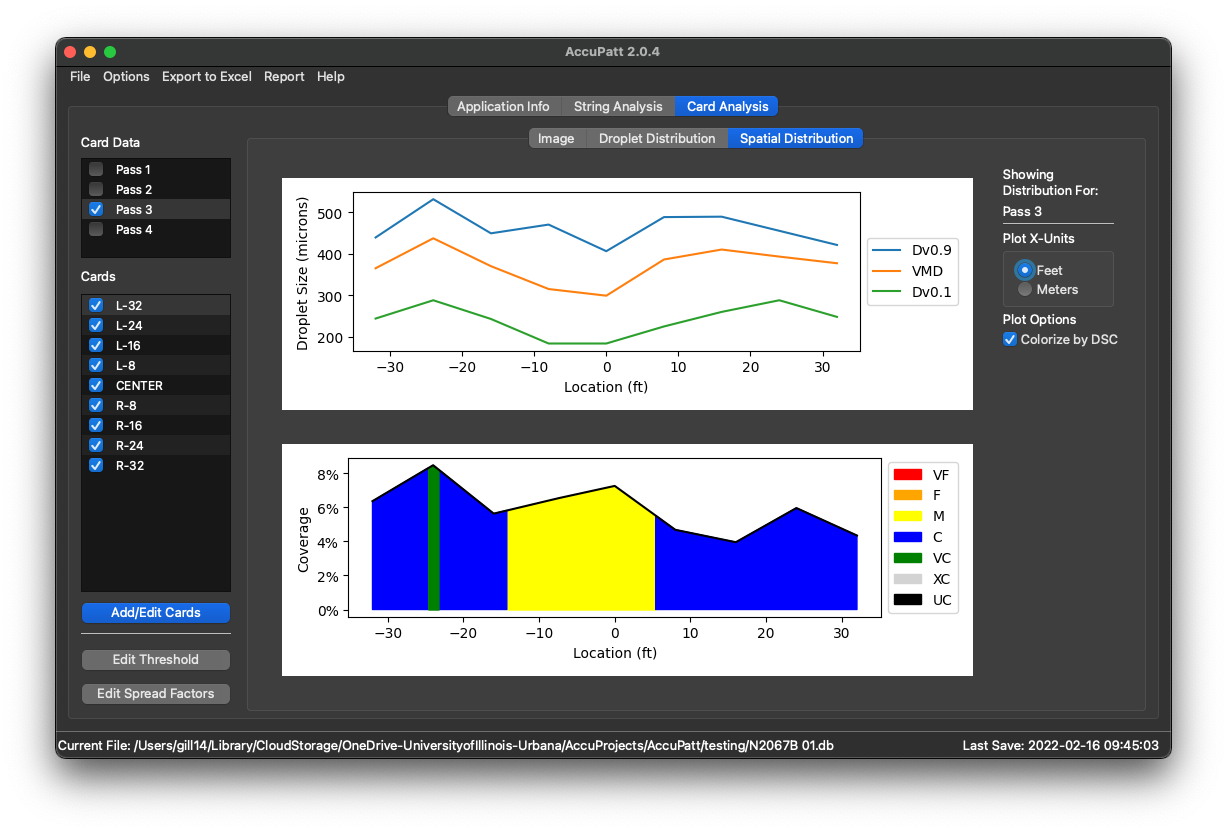
\includegraphics[width=\textwidth]{card_spatial_dist.png}}
        \caption{Spray-Card Analysis - Spatial Distribution}
        \label{fig:card_spatial_dist}
    \end{figure}
    \newpage

    \section{Spray-Card - Details}

    \subsection{Defined Sets}
    \label{sec:defined_sets}
    A convenience method for adding spray-cards to a pass is through the use of \textbf{Defined Sets} (Figure~\ref{fig:card_defined_set}). Navigate to the \textbf{Card Analysis} tab $\rightarrow$ \textbf{Add/Edit Cards} $\rightarrow$ \textbf{Define/Edit Sets}.\par
    A list of locally defined sets at the left can be modified via the \textbf{Add Set}, \textbf{Remove Set} and double-clicking the name to rename it. Selecting the set will populate the tableview at right with the cards in the set. Cards may be added, removed and shifted within the set via the respective buttons below the tableview.\par
    For regularly spaced cards, they may be added to the set in batch format by clicking the \textbf{Add Regularly Spaced Cards to Set} button (Figure~\ref{fig:card_defined_set_batch}). Given an initial location, quantity and either step distance or final location, a list of cards can be added to meet those requirements.\par
    All sets are stored on your local machine and will be available whenever you use the program.
    \begin{figure}[hb]
        \centering
        \makebox[\textwidth]{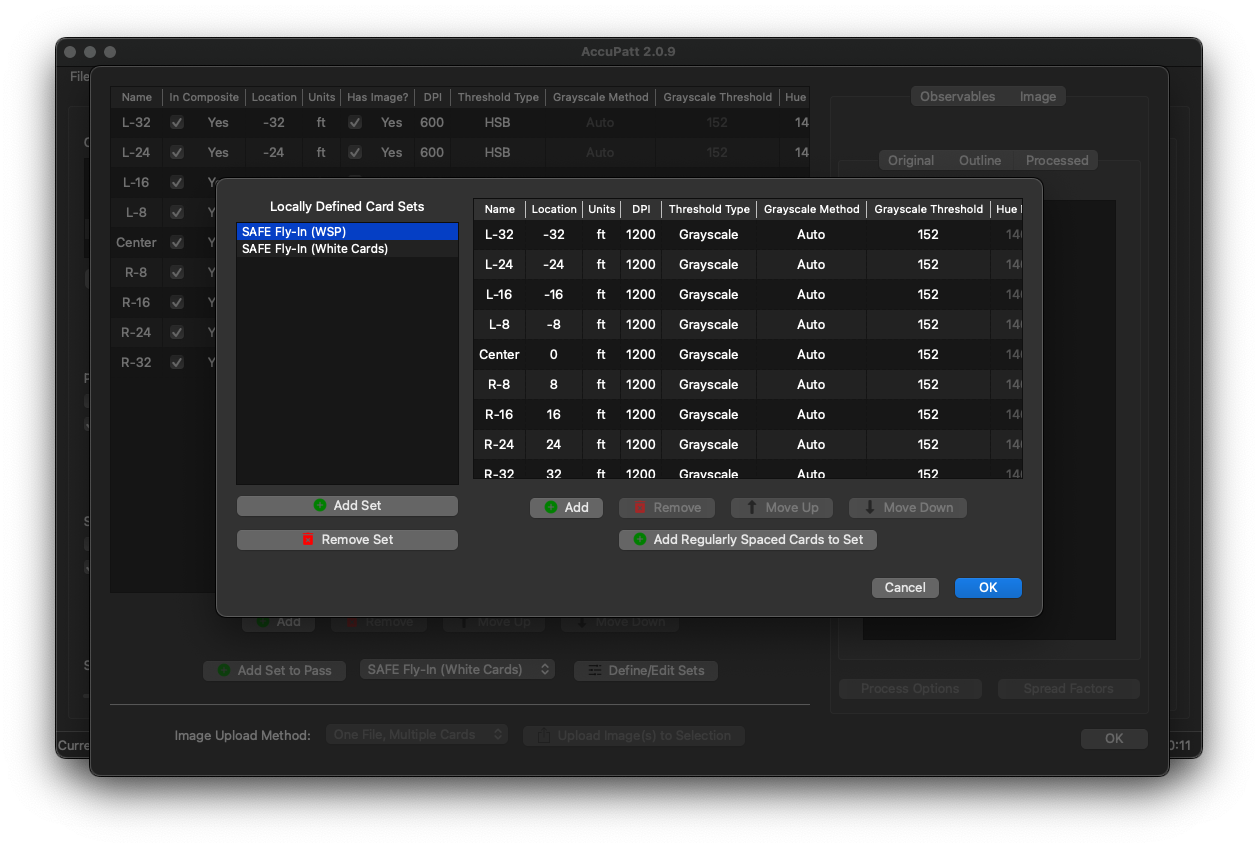
\includegraphics[width=\textwidth]{card_defined_set.png}}
        \caption{Spray-Card Analysis - Defined Set}
        \label{fig:card_defined_set}
    \end{figure}
    \begin{figure}[hb]
        \centering
        \makebox[\textwidth]{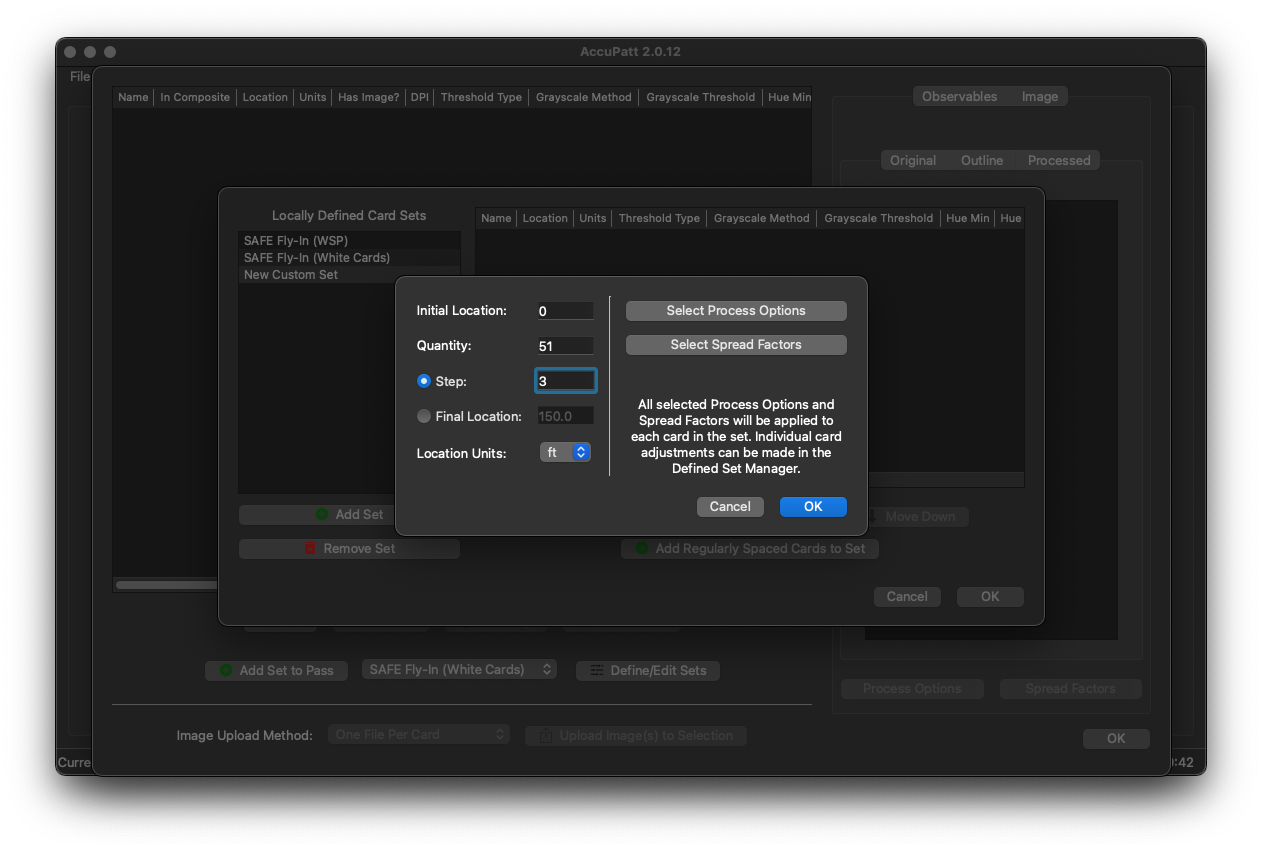
\includegraphics[width=\textwidth]{card_defined_set_batch.png}}
        \caption{Spray-Card Analysis - Defined Set - Add Batch}
        \label{fig:card_defined_set_batch}
    \end{figure}
    \FloatBarrier

    \subsection{Image Upload}
    \label{sec:image_upload}
    Images are uploaded to the datafile using the method selected in the \textbf{Image Upload Method} dropdown. With the cards you intend to upload selected in the Card Manager tableview, click \textbf{Upload Image(s) to Selection}. Note that image files must be of type \textit{*.png : Portable Network Graphics} or \textit{*.tif, *.tiff : Tagged Image File Format}. Ensure that images are acquired with no pre-processing, corrections, enhancements or compression.

    \subsubsection{One File, Multiple Cards}
    When multiple cards are acquired in a single large scan, this method will allow cropping of each card and saving individually to the datafile. After selecting the file, the image will be shown with each card's independently draggable, resizable region-of-interest (ROI) (Figure~\ref{fig:card_upload_multiple}). The image may be panned or zoomed-upon. To decrease RAM consuption, large images are shown in lower resolution here, but full-resolution ROI's will be cropped out of the original image using a scaled coordinate system. The following options are available to adjust the method for which these ROI's are drawn:
    \begin{itemize}
        \item \textbf{Pixels Per Inch:} Automatically set by the image metadata, but user-adjustable. This is used in conjunction with the image pixel dimensions to show calculated image dimensions. These are provided only to allow verification by the user of proper pixels per inch setting.
        \item \textbf{Orientation:} Used in conjunction with order to decide automatic assigning of names to cards. Either vertical or horizontal.
        \item \textbf{Order:} Used in conjunction with orientation to dictate automatic assigning of names to cards. Either Increaseing or decreasing.
        \item \textbf{Sampling Area:} After cards are located, the percentage of width and height to draw the rectangular ROI.
    \end{itemize}
    \begin{figure}[hb]
        \centering
        \makebox[\textwidth]{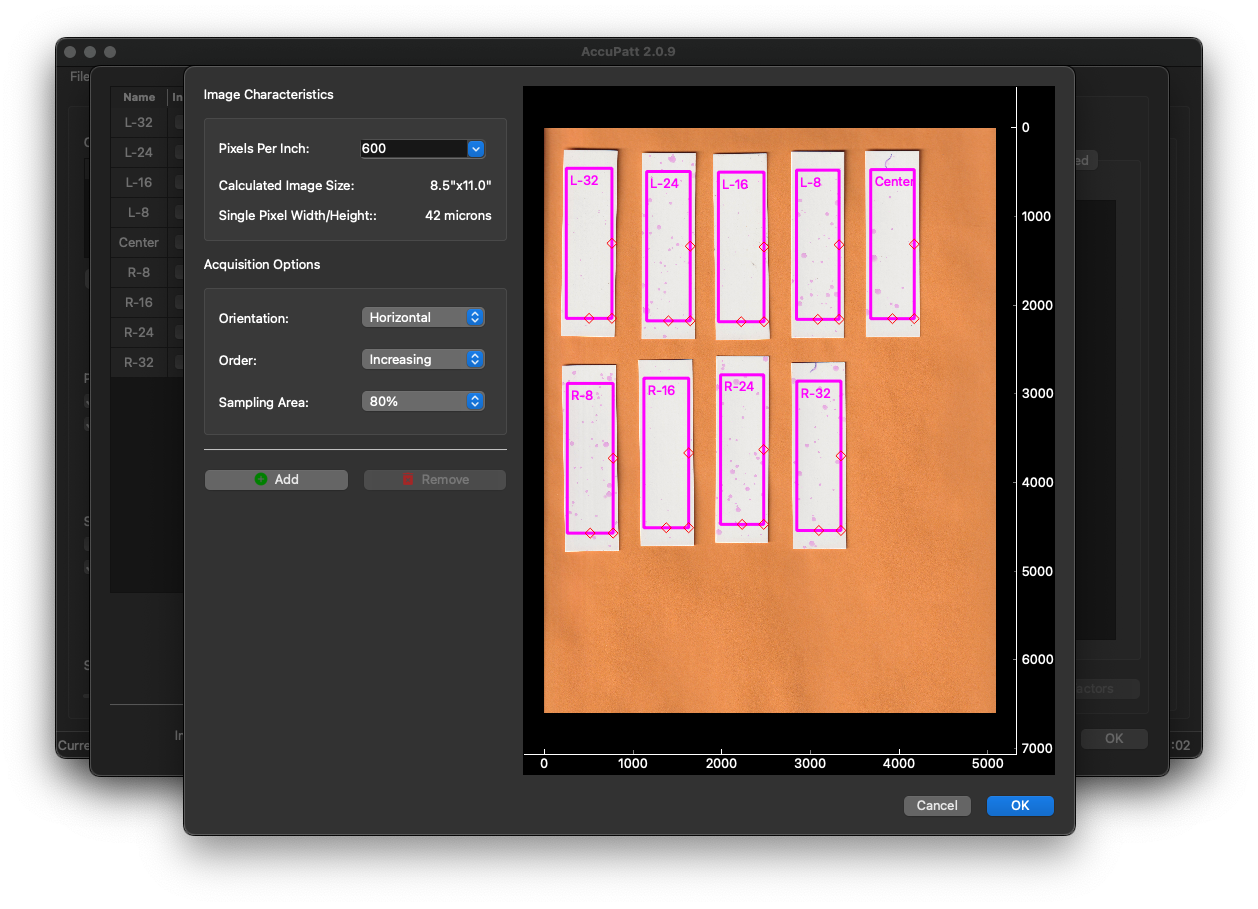
\includegraphics[width=\textwidth]{card_upload_multiple.png}}
        \caption{Spray-Card Analysis - Upload Image with Multiple Cards}
        \label{fig:card_upload_multiple}
    \end{figure}
    \FloatBarrier

    \subsubsection{One File per Card}
    For images which are already cropped appropriately, they can be directly uploaded to the datafile (Figure~\ref{fig:card_upload_singles}). Selected files can be dragged to alter the order to match the proper order of declared card names.
    \begin{figure}[hb]
        \centering
        \makebox[\textwidth]{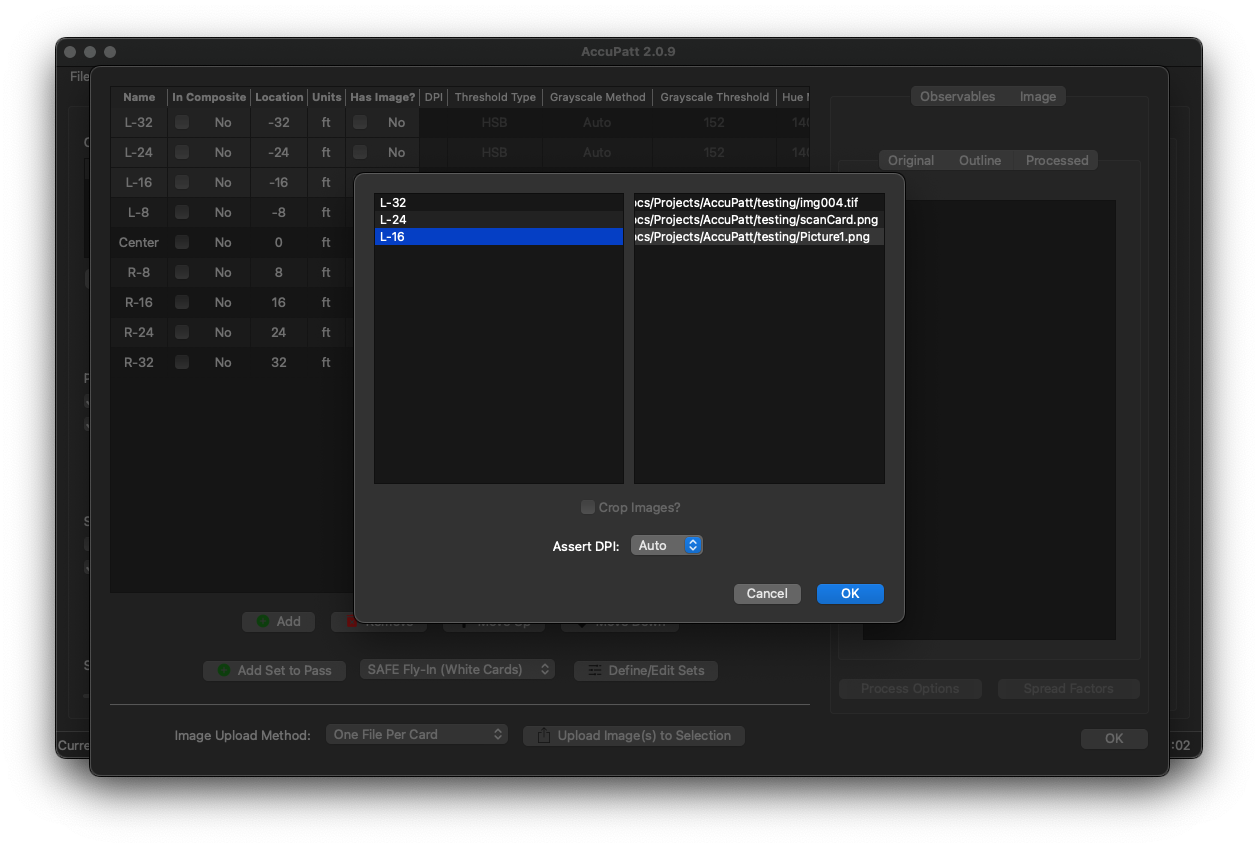
\includegraphics[width=\textwidth]{card_upload_singles.png}}
        \caption{Spray-Card Analysis - Upload Single Images}
        \label{fig:card_upload_singles}
    \end{figure}
    \FloatBarrier

    \subsection{Image Process Options}
    \label{sec:image_process}
    The \textbf{Image Process Options} window (Figure~\ref{fig:card_image_process}) is opened by selecting a card in the card list which has image data, and then clicking the \textbf{Edit Threshold} button. It contains the following options:
    \begin{itemize}
        \item \textbf{Threshold Type:} Dropdown menu to select the type of threshold to use when binarizing the imge. Options are HSB (Hue-Saturation-Brightness) or Grayscale. This choice will limit the threshold options as follows:
        \begin{itemize}
            \item \textbf{HSB:} Binarizes image by pixel filtering the color image by 8-bit ranges (0-255) of Hue, Saturation and Brightness. Once the ranges are set, choose whether to \textbf{include} pixels (count them as part of a stain) which meet the criteria or \textbf{exclude} them (treat them as background)
            \item \textbf{Grayscale:} Converts the image to an 8-bit (0-255) grayscale image, then uses a threshold value to binarize the image, where values below the threshold are treated as background and values above the threshold are treated as part of a stain. This threshold may be set manually, or automatically. The automatic method uses Otsu's Threshold Method, and is sufficient for most bimodal images.
        \end{itemize}
        \item \textbf{Watershed Segmentation:} Attempt to seperate adjoining stains. \color{red} This is still a work in progress and should generally be kept disabled \color{black}
        \item \textbf{Stain Approximation:} After thresholding and segmentation, optionally attempt to transform each stain using the chosen method.
        \begin{itemize}
            \item \textbf{Minimum Enclosing Circle:} Draw the smallest circle possible which contains the stain.
            \item \textbf{Fit Ellipse:} Enclose the stain in the smallest possible rotated rectangle; draw the largest ellipse possible within it. Stain contours with less than 5 perimeter points are left unchanged.
            \item \textbf{Convex Hull:} Expand the stain such that there is no convexity defects (concave regions) between any perimeter points.
        \end{itemize}
        \item \textbf{Minimum Stain Size:} integer area in pixels below which stains should be treated as background.
    \end{itemize}
    By default, options are saved only to the selected card. Checking the \textbf{Apply To All} option of \textbf{Pass} or \textbf{Series} prior to saving will apply the options set to all applicable other cards and save that to the datafile. Additionally, checking \textbf{Update defaults with selection} will cause any spray cards created in the future to utilize these settings by default.
    
    \begin{figure}[hb]
        \centering
        \makebox[\textwidth]{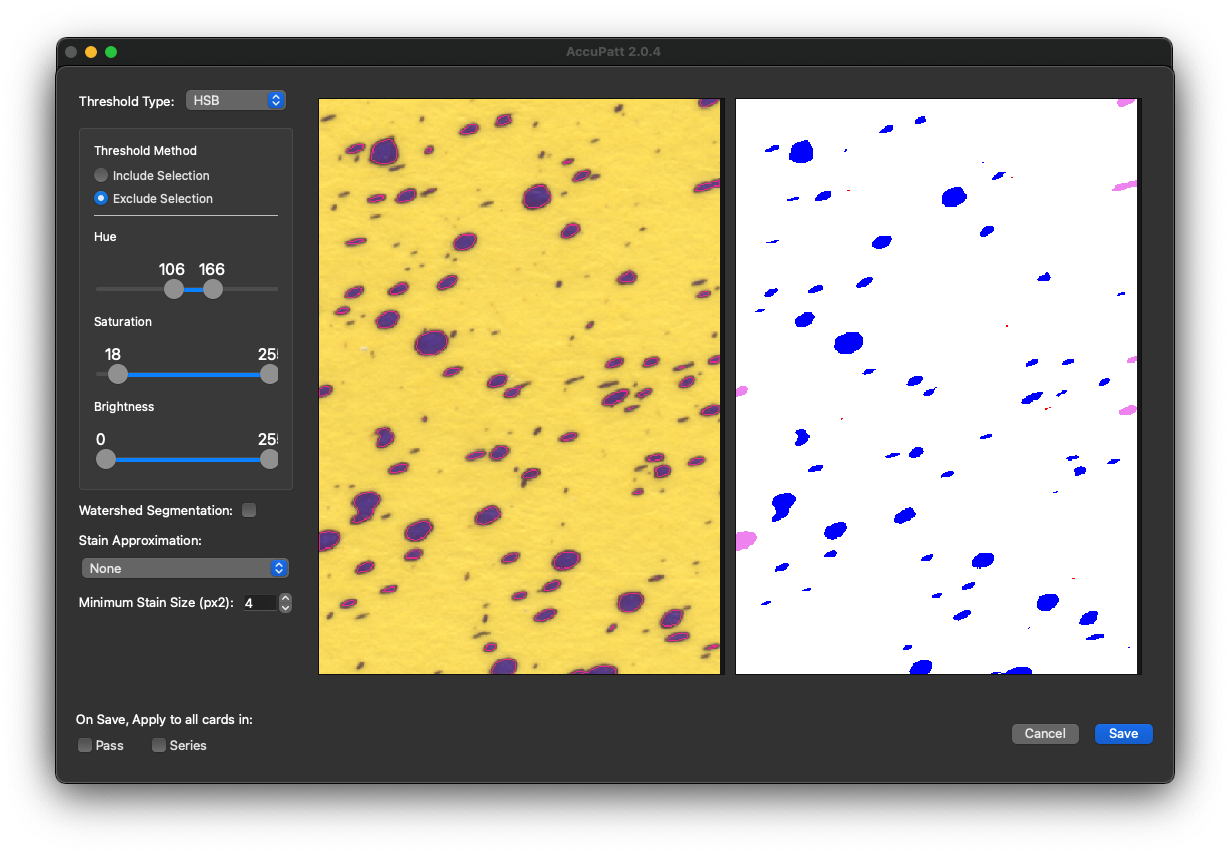
\includegraphics[width=\textwidth]{card_image_process.png}}
        \caption{Spray-Card Analysis - Image Process Options}
        \label{fig:card_image_process}
    \end{figure}
    \FloatBarrier

    \subsection{Stain to Droplet Calculation}
    \label{sec:spread_factors}
    The \textbf{Spread Factors} window (Figure~\ref{fig:card_spread_factors}) is opened by selecting a card in the card list which has image data, and then clicking the \textbf{Spread Factors} button. Spread Factor Equations are optionally applied to estimate the droplet size (Droplet Diameter, $D_D$) which created a given stain (Stain Diameter, $D_S$). The Stain Diameter is determined from the circle of equal projection area of the stain. Two equation types are provided, with adjustable spread factors (\textbf{a}, \textbf{b} and \textbf{c} coefficients):
    \begin{itemize}
        \item \textbf{Adaptive:} $D_D = D_S / (aD_S^2+bD_S+cD_S)$
        \item \textbf{Direct:} $D_D = aD_S^2+bD_S+cD_S$
    \end{itemize}
    By default, options are saved only to the selected card. Checking the \textbf{Apply To All} option of \textbf{Pass} or \textbf{Series} prior to will apply the options set to all applicable other cards and save that to the datafile. Additionally, checking \textbf{Update defaults with selection} will cause any spray cards created in the future to utilize these settings by default.
    \begin{figure}[hb]
        \centering
        \makebox[\textwidth]{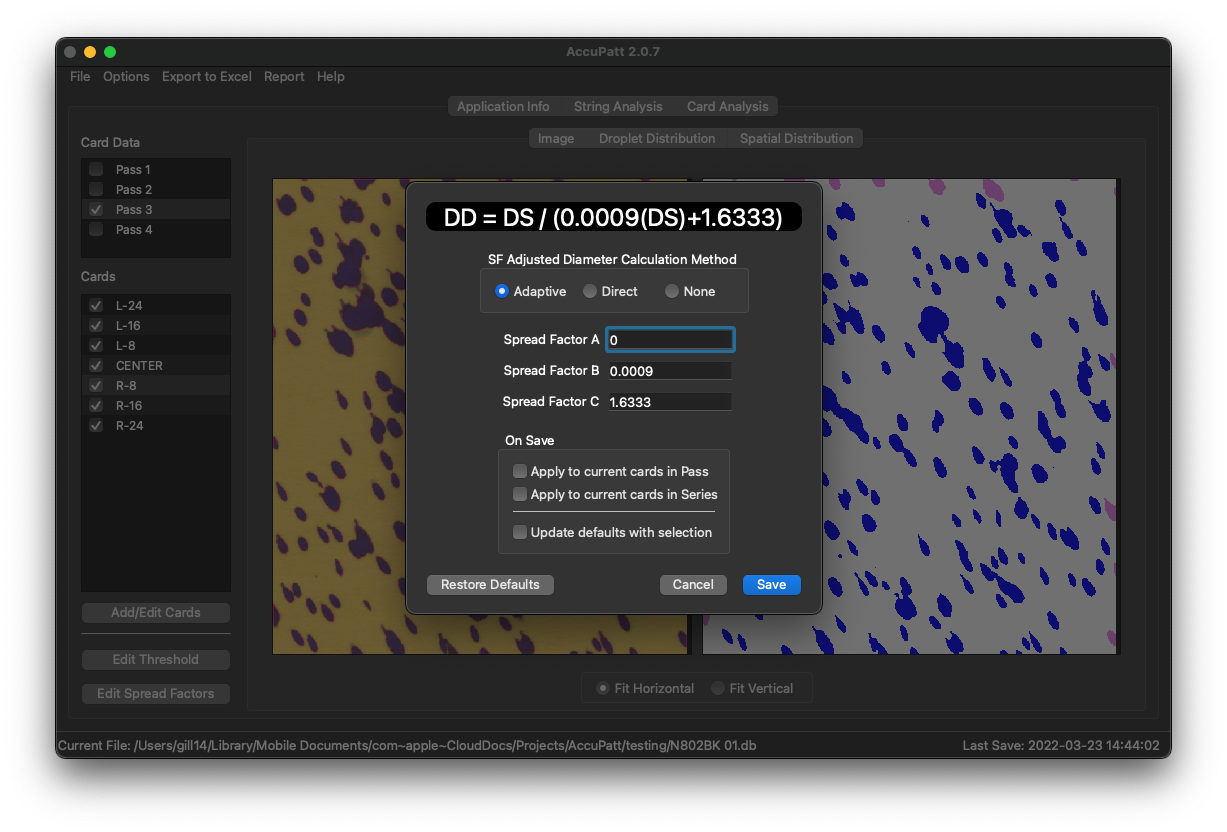
\includegraphics[width=\textwidth]{card_spread_factors.png}}
        \caption{Spray-Card Analysis - Spread Factors}
        \label{fig:card_spread_factors}
    \end{figure}
    \FloatBarrier

    \newpage

    \section{String Hardware System Settings}
    \label{sec:string_hardware_settings}

    \subsection{String Drive}
    From the \textbf{Capture/Edit Pass} window, string drive settings can be adjusted by clicking the \textbf{Edit String Drive} button, which opens the applicable window (Figure~\ref{fig:string_drive_settings}). This window contains a dropdown for choosing a serial communication port, and accompanying refresh button to re-populate this list (for example, if a device is plugged-in after opening this window). With a port chosen in the list, that port's manufacturer and product information will be displayed.\par
    There are two fields which allow setting of the \textbf{String Length} and \textbf{String Forward Speed}. The units of string length [ft or m] can also be set here, and this will trigger the units of string forward speed [ft/sec or m/sec] to follow. While the string forward speed can be set manually here, this can also be calculated interactively; Clicking the \textbf{Calculate String Speed} button will open the applicable window (Figure~\ref{fig:string_drive_speed}). Here, a known length of string will be advanced through the string drive. This length does not need to be equal to what is used for the flightline length. Clicking the \textbf{Start} button will begin advancing string and start a timer. Once the known length of string has passed through the string drive, clicking \textbf{Stop} will stop the string drive and timer and calculate the speed [known-length / elapsed-time]. Clicking \textbf{Ok} will save this speed and return to the \textbf{Edit String Drive} window.\par
    A \textbf{Direct Command} interface is included to facilitate querying and setting string drive stepper motor paramaters to onboard nonvolatile memory. The Take-Up Reel corresponds to address \textbf{A} and the Supply Reel corresponds to address \textbf{B}. With a command typed into the textfield, clicking the \textbf{Send} button will append a carriage return, encode the message and send it to the stepper motor driver. A string of return text is normally recieved, and is displayed when available. This return text may simply be an echo of your command, or it may contain paramater information. See the stepper motor driver documentation by clicking the \textbf{?} button for specific commands.
    \begin{figure}[hb]
        \centering
        \makebox[\textwidth]{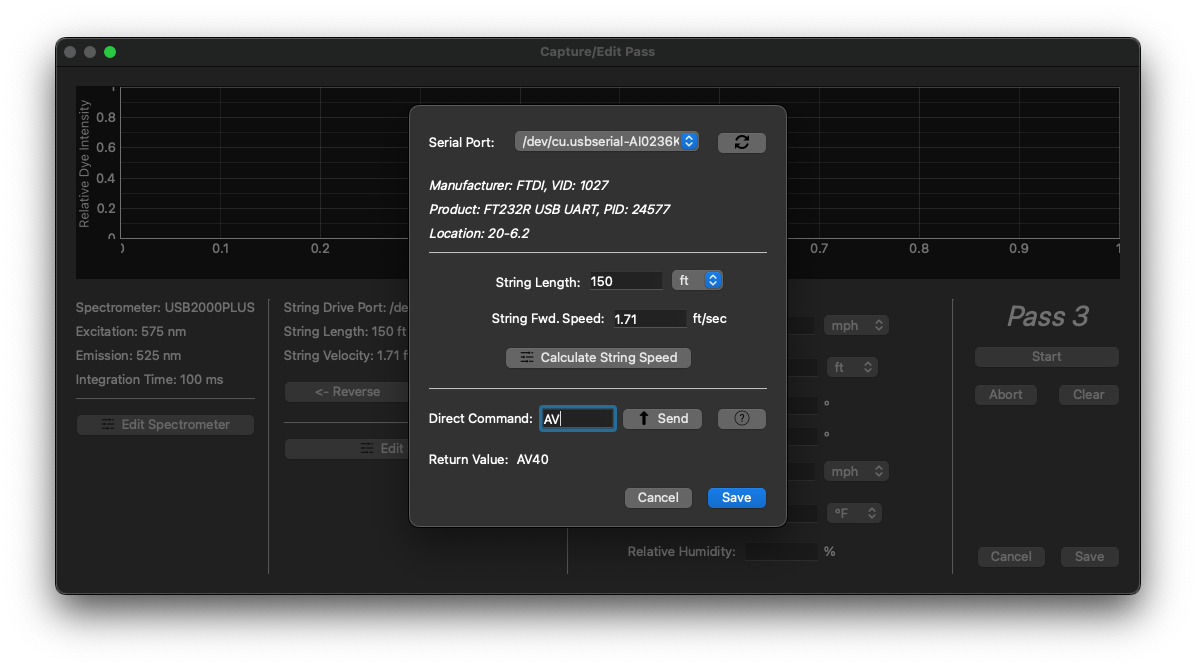
\includegraphics[width=0.75\textwidth]{string_drive_settings.png}}
        \caption{String Drive Settings}
        \label{fig:string_drive_settings}
    \end{figure}
    \begin{figure}[hb]
        \centering
        \makebox[\textwidth]{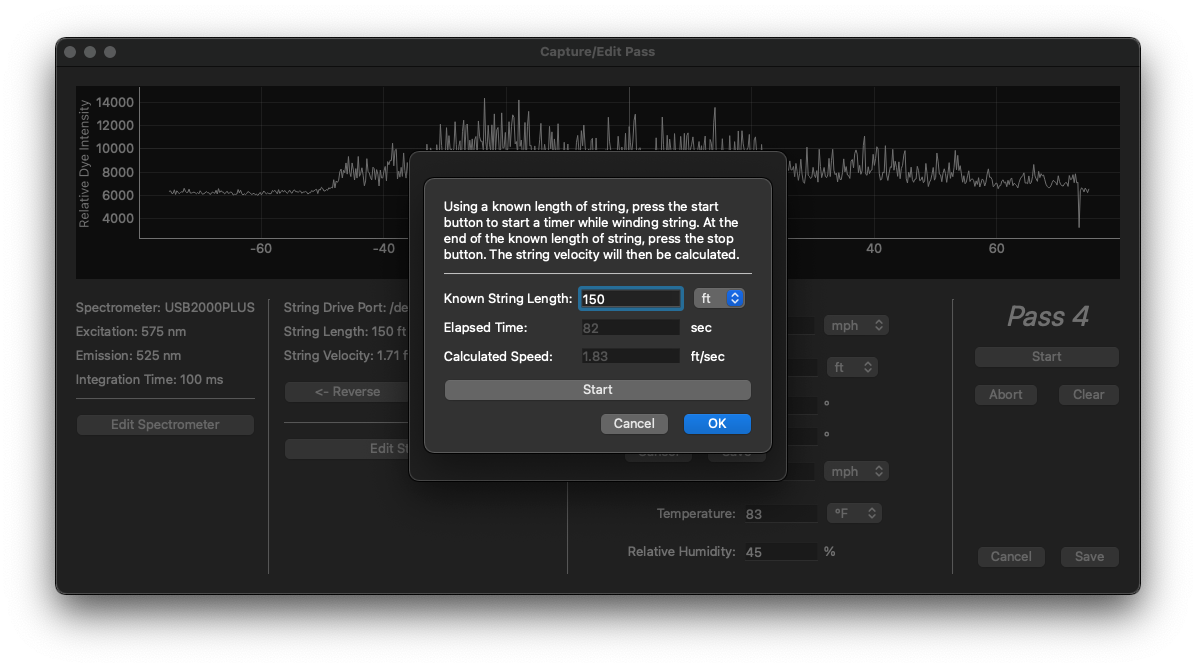
\includegraphics[width=0.75\textwidth]{string_drive_speed.png}}
        \caption{Interactively Calculate String Drive Speed}
        \label{fig:string_drive_speed}
    \end{figure}
    \FloatBarrier

    \subsection{Spectrometer}
    From the \textbf{Capture/Edit Pass} window, spectrometer settings can be adjusted by clicking the \textbf{Edit Spectrometer} button, which opens the applicable window (Figure~\ref{fig:spectrometer_settings}). This window displays the currently connected spectrometer's model and serial numbers. An accompanying refresh button is included to re-scan for a spectrometer (for example, if one is plugged-in after opening this window).\par
    There are three fields which allow setting of the \textbf{Excitation Wavelength (nm)}, \textbf{Emission Wavelength (nm)} and \textbf{Integration Time (milliseconds)}. The chosen wavelengths do not change the operation of the spectrometer; a full spectrum reading is always provided. They merely change the points on the spectrum from which this software collects and displays data. Note that each spectrometer is calibrated differently, and this software will attempt to find the pixel on the spectrometer which corresponds to the wavelength closest to that specified. This pixel and actual wavelength is displayed here. The integration time set here is sent to the spectrometer and does change its operation. Briefly, consider the integration time as the exposure on a camera; longer times correspond with more detail incorporated in each data frame, but a lower quantity of data frames per unit length of string. Clicking \textbf{Ok} will save these settings and return to the \textbf{Capture/Edit Pass} window.
    \begin{figure}[hb]
        \centering
        \makebox[\textwidth]{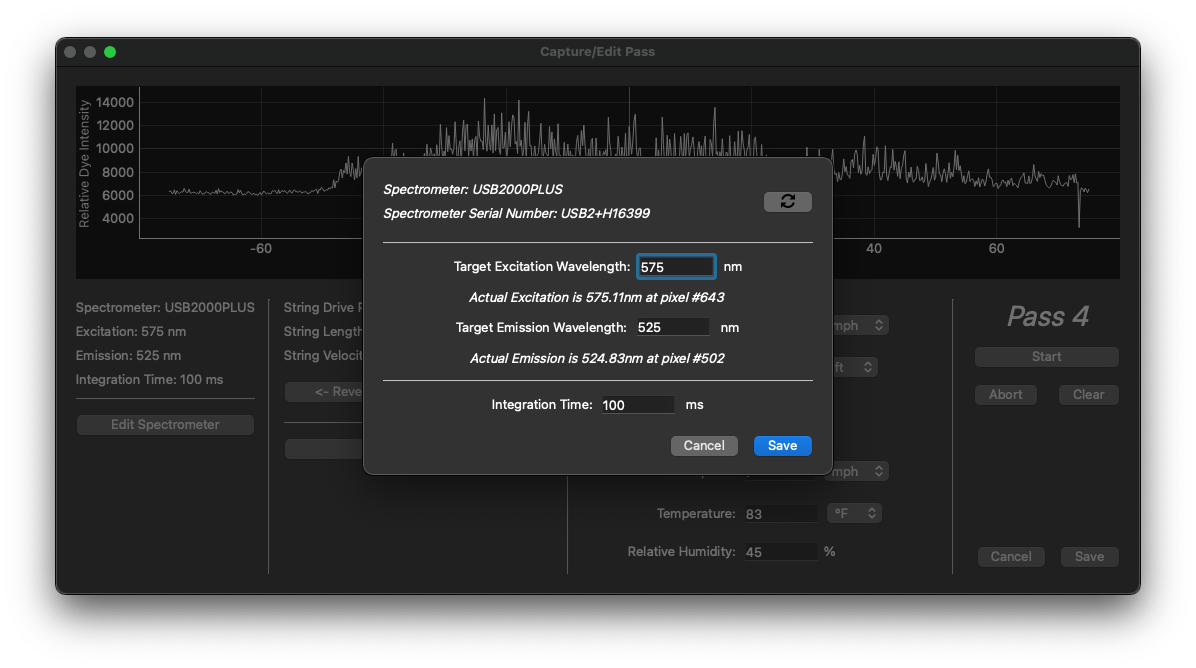
\includegraphics[width=0.75\textwidth]{spectrometer_settings.png}}
        \caption{Spectrometer Settings}
        \label{fig:spectrometer_settings}
    \end{figure}
    \FloatBarrier
    \newpage

    \section{Creating PDF Reports}
    Creating a printable/distributable report is a key function, and \textit{AccuPatt} provides utility to generate various report permuations using the \textit{Portable Document Format (*.pdf)}. The following options can be set from the \textbf{Report} menu:
    \begin{itemize}
        \item \textbf{Include Card Images:} [True/False] Whether to add page(s) to the report with individual card images/statistics.
        \item \textbf{Card Image Type:} [Original, Outline, Mask] What type of image to use in report.
        \item \textbf{Card Images Per Page:} [5, 7, 9] Card images are scaled to fit, so this effectively allows balancing desired image size and resultant number of pages required.
    \end{itemize}

    \subsection{Operation S.A.F.E. Report}
    Creates a standardized report with the following pages:
    \begin{itemize}
        \item \textbf{String Summary Page:} Headers with all reported application info and observables. Plots overlay, average and simulations. Includes a uniformity (Coefficient of Variation) table. Page will only be included if at least one string pass is collected and selected for inclusion in the composite.
        \item \textbf{Card Summary Page:} Headers with all reported application info and observables. Plots Volume Fraction by location, coverage and droplet spectrum category by location, spray volume by droplet diameter and number of droplets by droplet diameter. Pass-wise droplet spectrum characteristics are shown for measured data as well as a USDA Model simulation for the provided nozzle/observable parameters. One page will be included for each pass which has card data associated with it and is selected for inclusion in the composite.
        \item \textbf{Card Image Page:} Individual card images displayed as per the report settings. Individual card statistics shown below each card. Pages included for each pass which has card data associated with it and is selected for inclusion in the composite. Number of pages required will vary based on number of cards and report options selected.
    \end{itemize}
    \newpage

    \section{Exporting Data to Excel}
    While typically unnecessary, it is sometimes desirable to export data obtained in \textit{AccuPatt} into a format more widely accesible. To facilitate this, data can be copied to a \textit{Microsoft Excel (*.xlsx)} file by choosing one of the following options from the \textbf{Export} menu:
    \begin{itemize}
        \item \textbf{Operation S.A.F.E. Attendee Log:} Prompts selection of any number of data files, and generates the file required by NAAREF to document attendance at a S.A.F.E. Fly-In.
        \item \textbf{All Raw Data:} Exactly like it sounds, no processing or calculations, just the data and parameter settings.
        \item \textbf{Processed Data:} \color{red} To-Do \color{black}
        \item \textbf{All Images:} \color{red} To-Do \color{black}
    \end{itemize}
    \newpage

    \section{Opening Past Datafiles}
    From the menubar choose \textbf{File $\rightarrow$ Open} to open a filechooser window and select the file to open. Legacy files created in AccuPatt 1.xx, when opened, will cause a choice prompt to open the file as \textbf{View Only} or to \textbf{Create Compatible Copy} (Figure~\ref{fig:open}). If the latter is chosen, an identically named .db file will be placed in the same directory as the original file. The original (.xlsx) file is never edited, only read.
    \begin{figure}[hb]
        \centering
        \makebox[\textwidth]{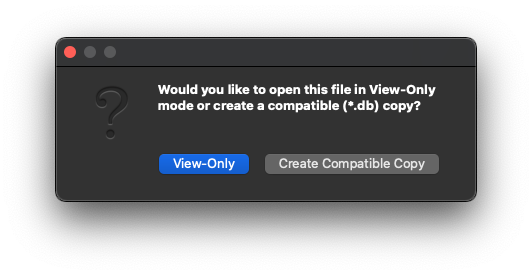
\includegraphics[width=0.75\textwidth]{open.png}}
        \caption{Open Datafile}
        \label{fig:open}
    \end{figure}
    \newpage

    \section{Data Structure}
    \label{sec:data}
    To the greatest extent practical, all provided analysis options are persistent for a saved data file. This is to ensure that, when re-opened at a later date or on another computer, results will be as close to identical as possible. Below is a relational outline for a data file.
    \begin{itemize}
        \item \textbf{series-id:} unique identifier, automatically generated.
        \item \textbf{series-number:} integer
        \item \textbf{flyin:}
        \begin{itemize}
            \item \textbf{name:} text
            \item \textbf{location:} text
            \item \textbf{date:} integer, unix timestamp
            \item \textbf{analyst:} text
        \end{itemize}
        \item \textbf{applicator:} 
        \begin{itemize}
            \item \textbf{pilot:} text
            \item \textbf{business:} text
            \item \textbf{street:} text
            \item \textbf{city:} text
            \item \textbf{state:} text
            \item \textbf{zip:} text
            \item \textbf{phone:} text
            \item \textbf{email:} text
        \end{itemize}
        \item \textbf{aircraft:} 
        \begin{itemize}
            \item \textbf{registration:} text
            \item \textbf{make:} text
            \item \textbf{model:} text
            \item \textbf{wingspan:} float, units=[ft, m]
            \item \textbf{winglets:} true/false
        \end{itemize}
        \item \textbf{spray-system:} 
        \begin{itemize}
            \item \textbf{swath-target:} float, units=[ft, m]
            \item \textbf{swath-adjusted:} float
            \item \textbf{rate-target:} float, units=[gpa, l/ha]
            \item \textbf{boom-pressure:} float, units=[psi, bar, kpa]
            \item \textbf{boom-width:} float, units=[ft, m]
            \item \textbf{boom-drop:} float, units=[in, cm]
            \item \textbf{nozzle-spacing:} float, units=[in, cm]
        \end{itemize}
        \item \textbf{nozzles:} [list]
        \begin{itemize}
            \item \textbf{type:} text
            \item \textbf{size:} text
            \item \textbf{deflection:} text
            \item \textbf{quantity:} integer
        \end{itemize}
        \item \textbf{notes-setup:} text
        \item \textbf{notes-analyst:} text, will not print on reports
        \item \textbf{string-settings:} 
        \begin{itemize}
            \item \textbf{equalize-integrals:} true/false, scale all passes to largest integrated area
            \item \textbf{average-center:} true/false, apply average-center-method
            \item \textbf{average-center-method:} text, option=[centroid, center-of-distribution]
            \item \textbf{average-smooth:} true/false, apply smoothing filter to average pattern
            \item \textbf{average-smooth-window} float, x-domain window over which to apply smoothing
            \item \textbf{average-smooth-order} integer, polynomial order for smoothing filter
            \item \textbf{number-simulated-adjascent-passes:} integer, per-side basis
        \end{itemize}
        \item \textbf{passes:} [list]
        \begin{itemize}
            \item \textbf{pass-id:} unique identifier, automatically generated
            \item \textbf{name:} editable text, default is 'Pass ' + position in passes list at creation
            \item \textbf{string-include-in-composite:} True/False, include pass in series-wise calculations/plots
            \item \textbf{cards-include-in-composite:} True/False, include pass in series-wise calculations/plots
            \item \textbf{observables:} 
            \begin{itemize}
                \item \textbf{ground-speed:} float, units=[mph, kph, kn]
                \item \textbf{spray-height:} float, units=[ft, m]
                \item \textbf{pass-heading:} integer, range=[0-359]
                \item \textbf{wind-direction:} integer, range=[0-359]
                \item \textbf{wind-speed:} float, units=[mph, kph, kn]
                \item \textbf{temperature:} float, units=[\degree F, \degree C]
                \item \textbf{humidity:} float
            \end{itemize}
            \item \textbf{string:} 
            \begin{itemize}
                \item \textbf{wavelength-excitation:} integer, units=[nm]
                \item \textbf{wavelength-emission:} integer, units=[nm]
                \item \textbf{integration-time:} integer, units=[ms]
                \item \textbf{data-excitation:} list[float, float], [location, intensity]
                \item \textbf{data-emission:} list[float, float], [location, intensity]
                \item \textbf{data-location-units:} units=[ft, m]
                \item \textbf{trim-left:} integer, number of sample points to set to floor value
                \item \textbf{trim-right:} integer, number of sample points to set to floor value
                \item \textbf{trim-vertical:} float, value to subtract from all points in addition to floor value
                \item \textbf{rebase:} true/false, use trim-l/trim-r to scale x-domain 
                \item \textbf{center:} true/false, apply center-method to pass
                \item \textbf{center-method:} text, option=[centroid, center-of-distribution]
                \item \textbf{smooth:} true/false, apply smoothing filter to pass
                \item \textbf{smooth-window} float, x-domain window over which to apply smoothing
                \item \textbf{smooth-order} integer, polynomial order for smoothing filter
            \end{itemize}
            \item \textbf{spray-cards:} [list]
            \begin{itemize}
                \item \textbf{id:} unique identifier, automatically generated
                \item \textbf{name:} text
                \item \textbf{include-in-composite} true/false, include spray-card in pass-wise calculations/plots
                \item \textbf{location:} float, optional linear location of spray-card, units=[ft,m]
                \item \textbf{ppi:} integer, image resolution in pixels per inch, symmetric only
                \item \textbf{threshold-type:} text, options=[grayscale, hue-saturation-brightness]
                \item \textbf{threshold-grayscale-method:} text, options=[automatic, manual]
                \item \textbf{threshold-grayscale:} integer, range=[0-255]
                \item \textbf{threshold-hsb-method:} text, options=[include-selection, exclude-selection]
                \item \textbf{threshold-hsb-hue-range:} [integer, integer], range=[0-255]
                \item \textbf{threshold-hsb-saturation-range:} [integer, integer], range=[0-255]
                \item \textbf{threshold-hsb-brightness-range:} [integer, integer], range=[0-255]
                \item \textbf{watershed:} true/false, stain segmentation using euclidian distance map
                \item \textbf{min-stain-area:} integer, minimum square pixel area to count as stain
                \item \textbf{stain-approximation-method:} text, options=[none, min-enclosing-circle, fit-ellipse, convex-hull]
                \item \textbf{spread-factor-equation:} text, options=[none, direct, adaptive]
                \item \textbf{spread-factor-a:} float
                \item \textbf{spread-factor-b:} float
                \item \textbf{spread-factor-c:} float
                \item \textbf{image:} image, limited to *.png *.tif *.tiff
            \end{itemize}
        \end{itemize}
    \end{itemize}

    \newpage

    \section{Changelog}
    \begin{itemize}
        \item \textbf{2.0.8 - 24 Mar 2022}
        \begin{itemize}
            \item (fix) Droplet stat table inadvertently defaulting to persistent dpi
            \item (fix) Import AccuPatt 1 cards inadvertently defaulting to persistent dpi
            \item (feature) Rebuild Pass Manager for pass observables
            \item (feature) Set default number of passes in Pass Manager
            \item (feature) Impose units for series-wise observable means
            \item (feature) Impose units for retrieving pass observables
            \item (feature) Add cards-include-in-composite to Pass for series-wise calculations
            \item (feature) String Drive - Direct Command Line
            \item (feature) User-defined defaults for string advanced options
            \item (feature) User-defined defaults for spray card processing and spread factors
            \item (feature) *.tif *.tiff support for loading spray cards
        \end{itemize}
        \item \textbf{2.0.7 - 16 Mar 2022}
        \begin{itemize}
            \item (fix) Spectrometer disconnect on subsequent calls to capture string
            \item (fix) Atomization model pressure/airspeed unit prechecks
            \item (fix) Duplicate labels on Card Manager table item delegates
            \item (feature) Fully adjustable (editable) DPI, in addition to suggested list
            \item (feature) Add SprayCard individual images/statistics pages to SAFE Report
            \item (feature) Report Menu - New Item: Include SprayCard images
            \item (feature) Report Menu - New Item: SprayCard image type
            \item (feature) Report Menu - New Item: SprayCard images per page
            \item (feature) Options Menu - New Item: Reset all user-defined defaults
        \end{itemize}
        \item \textbf{2.0.6 - 14 Mar 2022}
        \begin{itemize}
            \item (fix) Capture String window string data/option migrations
            \item (fix) Serial port handoffs between dialogs
            \item (feature) String Advanced Options dialog for pass/series smoothing and centering params
            \item (feature) String simulation view option: one-pass/all-passes
        \end{itemize}
        \item \textbf{2.0.5 - 11 Mar 2022}
        \begin{itemize}
            \item (fix) Replaced implicit dtypes on persistent settings with explicit dtypes for Windows
            \item (fix) Multiple plot and table reformats 
            \item (feature) String pattern x-mods now apply directly rather than using nearest point shift
            \item (feature) String pattern rebase (allows adjustment of x-domain post-processing)
            \item (feature) String pattern centering boolean and center-method replaces standalone method
            \item (feature) String pattern smoothing window/order moved to persistent settings
            \item (feature) String pattern smoothing window now x-domain-based rather than point-based 
            \item (feature) String pattern smooth/rebase now affects individual trim plot
            \item (feature) Auto-open report PDF upon generation
        \end{itemize}
        \item \textbf{2.0.4 - 25 Feb 2022}
        \begin{itemize}
            \item (fix) String Simulation mean deposition line
            \item (fix) Multiple plot legend fixes
            \item (feature) SAFE Report - Added spray card page(s)
            \item (feature) Locally Defined Card Sets, Batch Creator
            \item (feature) Batch Image Upload functionality
            \item (feature) Set image dpi by default from queried exif data
            \item (feature) Image Processing stain shape approximation
            \item (feature) Duplicate Pass observables from Capture String Pass to Card Manager
            \item (feature) Add persistence to Pass and Spray-Card options
            \item (feature) Add some non-model nozzles for convenience
            \item (feature) Add fly-in worksheets to help menu for convenience
            \item (feature) Add version number to datafile, window title and about popup
        \end{itemize}
        \item \textbf{2.0.3 - 2 Feb 2022}
        \begin{itemize}
            \item (fix) Remove SS/Def Atomization Model redundancies from Nozzle Selection
            \item (fix) Atomization Model Prechecks for airspeed, orifice, deflection and pressure
            \item (fix) String plot spatial units now follow target swath units, regardless of collection units
            \item (fix) Card plot spatial units now follow target swath units, regardless of collection units (override incl.)
            \item (feature) Excitation/Emission wavelengths and integration time saved to datafile
            \item (feature) Centering/Smoothing on per-pass basis
            \item (feature) Average Centering/Smoothing and Integral Equalization on series-basis
            \item (feature) Centering options: Centroid, Center of Distribution (Dr. Fritz)
            \item (feature) Spray Card min particle size, watershed segmentation optional
            \item (feature) Spray Card image processed colors seperated for edge (incl in cov) vs undersized stains (excl in cov)
            \item (feature) Fold importing of AccuPatt 1 files into standard open menu, with optional to view-only or create db copy
            \item (feature) Windows Installer
        \end{itemize}
        \item \textbf{2.0.2 - 28 Jan 2022}
        \begin{itemize}
            \item (feature) measure string speed
            \item (fix) save trigger before opening Card Manager
        \end{itemize}
        \item \textbf{2.0.1 - 27 Jan 2022}
        \begin{itemize}
            \item (fix) handling of blank spray cards
            \item (fix) parsing new string data to pass object
        \end{itemize}
        \item \textbf{2.0.0 - 26 Jan 2022} Initial Rewrite of AccuPatt. Final release of the legacy Java/JavaFX version is 1.06+. This rewrite uses Python/Qt.
    \end{itemize}

\end{document}